%%%%%%%%%%%%%%%%%%%%%%%%%%%%%%%%%%%%%%%%%%%%%%%%%%%%%%%%%%%%%%%%%%%%%%
% njuthesis 示例模板 v1.4.0 2024-03-19
% https://github.com/nju-lug/NJUThesis
%
% 贡献者
% Yu XIONG @atxy-blip   Yichen ZHAO @FengChendian
% Song GAO @myandeg     Chang MA @glatavento
% Yilun SUN @HermitSun  Yinfeng LIN @linyinfeng
%
% 许可证
% LaTeX Project Public License(版本 1.3c 或更高)
%%%%%%%%%%%%%%%%%%%%%%%%%%%%%%%%%%%%%%%%%%%%%%%%%%%%%%%%%%%%%%%%%%%%%%

%---------------------------------------------------------------------
% 一些提升使用体验的小技巧:
%   1. 请务必使用 UTF-8 编码编写和保存本文档
%   2. 请务必使用 XeLaTeX 或 LuaLaTeX 引擎进行编译
%   3. 不保证接口稳定,写作前一定要留意版本号
%   4. 以百分号(%)开头的内容为注释,可以随意删除
%---------------------------------------------------------------------

%---------------------------------------------------------------------
% 请先阅读使用手册:
% http://mirrors.ctan.org/macros/unicodetex/latex/njuthesis/njuthesis.pdf
%---------------------------------------------------------------------

\documentclass[
    % 模板选项:
    %
    % type = bachelor|master|doctor|postdoc, % 文档类型,默认为本科生
    % degree = academic|professional,        % 学位类型,默认为学术型
    %
    % nl-cover,   % 是否需要国家图书馆封面,默认关闭
    % decl-page,  % 是否需要诚信承诺书或原创性声明,默认关闭
    %
    %   页面模式,详见手册说明
    % draft,                  % 开启草稿模式
    % anonymous,              % 开启盲审模式
    % minimal,                % 开启最小化模式
    %
    %   单双面模式,默认为适合印刷的双面模式
    % oneside,                % 单面模式,无空白页
    % twoside,                % 双面模式,每一章从奇数页开始
    %
    %   字体设置,不填写则自动调用系统预装字体,详见手册
    % fontset = win|mac|macoffice|fandol|none,
  ]{njuthesis}

% 模板选项设置,包括个人信息、外观样式等
% 较为冗长且一般不需要反复修改,我们把它放在单独的文件里
% njuthesis 参数设置文件 v1.4.0 2024-03-19

% 一些提醒:
%   1. \njusetup 内部千万不要有空行
%   2. 使用英文半角逗号(,)分隔选项
%   3. 等于号(=)两侧的空格会被忽略
%       3.1. 为避免歧义,请用花括号({})包裹内容
%   4. 本科生无需填写的项目已被特别标注
%   5. 可以尽情删除本注释

% info 类用于录入个人信息
%   带*号的为对应英文字段
\njusetup[info]{
    title = {Rust语法结构与变更及错误倾向性关系实证研究},
    % 中文题目
    % 直接填写标题就是自动换行
    % 可以使用换行控制符(\\)手动指定换行位置
    %
    title* = {Empirical Study of relationship between Syntax Structures and Change- and Fault-proneness in Rust},
    % 英文题目
    %
    author = {张耀坤},
    % 作者姓名
    %
    author* = {ZHANG Yaokun},
    % 作者英文姓名
    % 一般使用拼音
    %
    keywords = {Rust程序设计语言,软件质量,变更倾向,错误倾向,语法项},
    % 中文关键词列表
    % 使用英文半角逗号(,)分隔
    %
    keywords* = {Rust programming language,software quality,Change proneness,Fault proneness,syntax items},
    % 英文关键词
    % 使用英文半角逗号(,)分隔
    %
    grade = {2020级},
    % 年级
    %
    student-id = {201220148},
    % 学号或工号
    % 研究生请斟酌大小写字母格式
    % 本模板并不会自动更正大小写
    %
    department = {计算机科学与技术系},
    department* = {Department of Computer Science and Technology},
    % 院系
    %
    major = {计算机科学与技术},
    major* = {Computer Science and Technology},
    % 专业
    %
    % major = {封面专业,摘要专业},
    % 研究生专业型学位可能遇到两处内容不一致的情况
    %
    supervisor = {冯洋,助理研究员},
    supervisor*= {Yang Feng,Assistant Researcher},
    % 导师全称
    % 使用英文半角逗号(,)分隔中文姓名和职称
    %
    % supervisor-ii = {第二导师姓名,副教授},
    % supervisor-ii* = {Associate professor My Second Supervisor},
    % 第二导师全称
    % 如果确实没有第二导师,不填写即可
    %
    submit-date = {2024-05-20},
    % 提交日期
    % 格式为 yyyy-mm-dd
    % 不填就是编译当天日期
    %
    %
    % 以下均为研究生项
    %
    % degree = {工程硕士},
    % degree* = {Master of Engineering},
    % 覆盖默认学位名称
    %
    field = {物理化学},
    field* = {Physical Chemistry},
    % 研究领域
    %
    chairman = {某某某~教授},
    % 答辩委员会主席
    % 推荐使用波浪号(~)分隔姓名和职称
    %
    reviewer = {
        某某某~教授,
        某某某~教授
    },
    %
    % 答辩委员会成员
    % 一般为四名,使用英文半角逗号(,)分隔
    %
    clc = {O643.12},
    % 中国图书分类号
    %
    udc = {544.4},
    % 国际图书分类号
    %
    secret-level = {公开},
    % 密级
    %
    defend-date = {2024-05-21},
    % 答辩日期
    % 格式为 yyyy-mm-dd
    % 不填就是编译当天日期
    %
    email = {201220148@smail.nju.edu.cn},
    % 电子邮箱地址
    % 只用于出版授权书
    %
    %
    % 以下用于国家图书馆封面
    confer-date = {2024-05-22},
    % 学位授予日期
    %
    bottom-date = {2024-05-23},
    % 封面底部日期
    %
    supervisor-contact = {
        南京大学~
        江苏省南京市栖霞区仙林大道163号
    }
    % 导师联系方式
}

% bib 类用于参考文献设置
\njusetup[bib]{
    % style = numeric|author-year,
    % 参考文献样式
    % 默认为顺序编码制(numeric)
    % 可选著者-出版年制(author-year)
    %
    resource = {njuthesis-sample.bib},
    % 参考文献数据源
    % 需要带扩展名的完整文件名
    % 可使用逗号分隔多个文件
    % 此条等效于 \addbibresource 命令
    %
    % option = {
        % doi    = false,
        % isbn   = false,
        % url    = false,
        % eprint = false,
        % 关闭部分无用文献信息
        %
        % refsection = chapter,
        % 将参考文献表置于每章后
        %
        % gbnamefmt = lowercase
        % 使用仅首字母大写的姓名
    %   }
    % 额外的 biblatex 宏包选项
}

% image 类用于载入外置的图片
\njusetup[image]{
    % path = {{./figure/}{./image/}},
    % 图片搜索路径
    %
    nju-emblem = {nju-emblem},
    nju-name = {nju-name},
    % 校徽和校名图片路径
    % 建议使用 PDF 格式的矢量图
    % 使用外置图片有助于减少编译时间
    % 空置时会自动使用 njuvisual 宏包绘制
    %
    % nju-emblem = {nju-emblem-purple},
    % nju-name = {nju-name-purple},
    % 替换为紫色版本
    % 这个选项只能填写一次
    % 切换时要注释掉上方的黑色版本
}

% abstract 类用于设置摘要样式
\njusetup[abstract]{
    toc-entry = false,
    % 摘要是否显示在目录条目中
    %
    % underline = false,
    % 研究生英文摘要页条目内容是否添加下划线
    %
    % title-style = strict|centered|natural
    % 研究生摘要标题样式,详见手册
}

% 目录自身是否显示在目录条目中
\njusetup{
    tableofcontents/toc-entry = false,
    % 关闭本项相当于同时关闭三个选项
    %
    % listoffigures/toc-entry   = false,
    % listoftables/toc-entry    = false
}

% 为目录中的章标题添加引导线
\njusetup[tableofcontents/dotline]{chapter}

% math 类用于设置数学符号样式,功能详见手册
\njusetup[math]{
    % style              = TeX|ISO|GB,
    % 整体风格,缺省值为国标(GB)
    % 相当于自动设置以下若干项
    %
    % integral           = upright|slanted,
    % integral-limits    = true|false,
    % less-than-or-equal = slanted|horizontal,
    % math-ellipsis      = centered|lower,
    % partial            = upright|italic,
    % real-part          = roman|fraktur,
    % vector             = boldfont|arrow,
    % uppercase-greek    = upright|italic
}

% theorem 类用于设置定理类环境样式,功能详见手册
\njusetup[theorem]{
    % define,
    % 默认创建内置的七种定理环境
    %
    % style         = remark,
    % header-font   = \sffamily \bfseries,
    % body-font     = \normalfont,
    % qed-symbol    = \ensuremath { \male },
    % counter       = section,
    % share-counter = true,
    % type          = {...}
    % 以上设置项在重新调用 theorem/define 后生效
}

% footnote 类用于设置脚注样式,功能详见手册
\njusetup[footnote]{
  % style = pifont|circled,
  % 使用圈码编号
  %
  % hang = false,
  % 不使用悬挂缩进
}

% 页眉页脚内容设置
\njusetup{
  % header/content = {
  %     {OR}{\thepage},{OL}{\rightmark},
  %     {EL}{\thepage},{ER}{\leftmark}
  %   },
  % 页眉设置,详见手册
  % 奇数页页眉:左侧章名,右侧页码
  % 偶数页页眉:左侧页码,右侧节名
  %
  % footer/content = {}
}

% 页眉页脚的字体样式
% \njusetformat{header}{\small\kaishu}
% \njusetformat{footer}{}

% 一些灵活调整
% \njusetname{type}{本科毕业设计}                 % 我做的是毕业设计
% \njusetname{notation}{术语表}                   % 更改符号表名称
% \njusetlength{crulewd}{240pt}                   % 加长封面页下划线
% \njusetformat{tabular}{\zihao{-4}\bfseries}     % 修改表格环境的字号
% \EditInstance{nju}{u/cover/emblem-img}{align=l} % 左对齐的本科生封面校徽


% 自行载入所需宏包
% \usepackage{subcaption} % 嵌套小幅图像,比 subfig 和 subfigure 更新更好
% \usepackage{siunitx} % 标准单位符号
% \usepackage{physics} % 物理百宝箱
% \usepackage[version=4]{mhchem} % 绘制分子式 
% \usepackage{algorithm,algorithmic} % 展示算法伪代码
\usepackage{listings}
\usepackage{parcolumns}
\usepackage{multicol} % 用于创建多栏布局
\usepackage{caption}  % 用于自定义图表标题
\usepackage{amsmath}
\usepackage{graphicx}
\usepackage{float} % 提供 H 选项
% \usepackage{xcolor}
\usepackage[table]{xcolor}
\usepackage{fancyvrb} % 解决 listings 和 minipage 的兼容性问题
\usepackage{algorithm}
\usepackage{algorithmicx}
\usepackage{algpseudocode}
\usepackage{array}
\usepackage{booktabs}
\usepackage{hyperref}

% 手动添加Rust语言支持
\lstdefinelanguage{Rust}{
  keywords={break, const, continue, crate, else, enum, extern, false, fn, for, if, impl, in, let, loop, match, mod, move, mut, pub, ref, return, self, Self, static, struct, super, trait, true, type, unsafe, use, where, while, async, await, dyn},
  keywordstyle=\color{blue}\bfseries,
  ndkeywords={bool, char, f32, f64, i8, i16, i32, i64, isize, str, u8, u16, u32, u64, usize, Option, Result, String, Vec},
  ndkeywordstyle=\color{cyan}\bfseries,
  identifierstyle=\color{black},
  sensitive=true,
  comment=[l]{//},
  morecomment=[s]{/*}{*/},
  commentstyle=\color{green}\ttfamily,
  stringstyle=\color{red}\ttfamily,
  morestring=[b]',
  literate=
    {'}{{\textquotesingle}}1
    {\\}{{\textbackslash}}1
}

\lstset{
language=Rust,
columns=fixed,       
numbers=left,                                        % 在左侧显示行号
numberstyle=\tiny\color{gray},                       % 设定行号格式
frame=none,                                          % 不显示背景边框
backgroundcolor=\color[RGB]{245,245,244},            % 设定背景颜色
keywordstyle=\color[RGB]{40,40,255},                 % 设定关键字颜色
numberstyle=\footnotesize\color{darkgray},           
commentstyle=\it\color[RGB]{0,96,96},                % 设置代码注释的格式
stringstyle=\rmfamily\slshape\color[RGB]{128,0,0},   % 设置字符串格式
showstringspaces=false,                              % 不显示字符串中的空格
breaklines=true,
}
\renewcommand\lstlistingname{代码示例}

% 在导言区随意定制所需命令
% \DeclareMathOperator{\spn}{span}
% \NewDocumentCommand\mathbi{m}{\textbf{\em #1}}

% 开始编写论文
\begin{document}

%---------------------------------------------------------------------
%	封面、摘要、前言和目录
%---------------------------------------------------------------------

% 生成封面页
\maketitle

% 文档默认使用 \flushbottom,即底部平齐
% 效果更好,但可能出现 underfull \vbox 信息
% 如需抑制这些信息,可以反注释以下命令
% \raggedbottom

\begin{abstract}
    Rust 是一种开源系统编程语言,旨在提供内存安全和线程安全,以解决 C 和 C++ 中常见的内存错误和并发问题。作为一种当下热门的编程语言,由它开发的软件质量备受关注。受过去几项研究的启发,我们试图对Rust 语法结构与软件变更及错误倾向性之间的关系展开研究,为此我们定义了四个研究问题,来探索 Rust 语言特性如何影响变更和错误倾向。
    
    我们选定了十二个流行的Rust项目作为研究对象,如 egui、iced、nushell、clap 等。对于变更倾向,我们通过设定的规则遍历版本控制系统中所有commit,将所有commit划分为变更commit和非变更commit;对于错误倾向,我们通过版本控制系统找到所有的错误修复commit,然后通过预先定义的算法搜索错误引入commit。对于如上收集到的commit,我们通过求解语法树编辑距离算法,获得我们关注的变动部分。分别使用优势比分析和逻辑回归分析对变动部分进行分析,得出研究结果。
    
    本研究发现,某些语法结构对软件变更和错误倾向有促进或者抑制作用。我们结合实际仓库对这些结论进行调查,分析了造成这些现象的原因,给出了讨论。另外,我们还分析这项研究的不足,并给出了对未来工作的展望。
\end{abstract}

\begin{abstract*}
    Rust is an open-source systems programming language designed to provide memory safety and thread safety, addressing common memory errors and concurrency issues found in C and C++. As a popular programming language today, the quality of software developed with Rust is highly regarded. Inspired by several previous studies, we aim to investigate the relationship between Rust's syntax structures and the propensity for changes and errors in software. To this end, we have defined four research questions to explore how Rust's language features influence change and error propensity.
    
    We selected twelve popular Rust projects as our research subjects, including egui, iced, nushell, clap, and others. For change propensity, we traversed all commits in the version control system using predefined rules, categorizing all commits into change commits and non-change commits. For error propensity, we identified all bug-fix commits from the version control system and used a predefined algorithm to search for bug-introducing commits. For the collected commits, we calculated the edit distance of syntax trees to focus on the changes of interest. We analyzed the changes using odds ratio analysis and logistic regression analysis to obtain our research results.
    
    This study found that certain syntax structures have a promotive or inhibitory effect on software changes and error propensity. We investigated these conclusions with actual repositories, analyzing the reasons behind these phenomena and providing a discussion. Additionally, we analyzed the limitations of this study and offered prospects for future work.
\end{abstract*}

% 生成目录
\tableofcontents
% 生成图片清单
% \listoffigures
% 生成表格清单
% \listoftables

%---------------------------------------------------------------------
%	正文部分
%---------------------------------------------------------------------
\mainmatter

% 符号表
% 语法与 description 环境一致
% 两个可选参数依次为说明区域宽度、符号区域宽度
% 带星号的符号表(notation*)不会插入目录
% \begin{notation}[10cm]
%   \item[DFT] 密度泛函理论 (Density functional theory)
%   \item[DMRG] 密度矩阵重正化群 (Density-Matrix Reformation-Group)
% \end{notation}

% 建议将论文内容拆分为多个文件
% 即新建一个 chapters 文件夹
% 把每一章的内容单独放入一个 .tex 文件
% 然后在这里用 \include 导入,例如
%   \chapter{引言}
\section{研究动机}

Rust 是一种开源系统编程语言,旨在提供内存安全和线程安全。它由Mozilla Research首次发布于2010年,以解决C和C++语言中常见的内存错误和并发问题。Rust 强调安全性和性能,其内存安全保证主要通过一种称为所有权(ownership)的系统实现,该系统无需垃圾收集器即可管理内存。

作为一门以安全为特点的系统级编程语言,其开发的软件质量备受关注。近年来,随着软件开发的复杂度日益增加,研究者们开始关注软件变更和错误倾向性。例如,在对Java语言的七个不同软件系统进行的一项研究中,通过分析软件的发展快照和构建马尔可夫模型,探索了设计模式和反模式之间的双向变异及其对软件质量的影响 \cite{kermansaravi2021investigating}。该研究发现,设计模式和反模式可以互相转变,某些特定的代码变更类型(如重命名、注释、声明和操作符的更改)主要触发这些模式的变异。更重要的是,这些变异在特定的上下文中更容易导致错误,为软件的设计模式转换和防止引入反模式提供了重要的视角。

另外还有Khomh等人在2012年的一项研究\cite{khomh2012exploratory},该研究深入分析了反模式对面向对象系统中类的变更和错误倾向性的影响。通过在ArgoUML、Eclipse、Mylyn和Rhino等软件系统的54个版本中检测到13种反模式,研究探讨了存在反模式的类与其他类相比,其变更或修复错误的可能性是否更高,这种可能性(如果更高)是否仅仅由于类的大小或反模式的存在,以及哪些类型的变更会影响参与反模式的类。

上述研究的发现对于Rust语言的研究具有启示意义。Rust作为一种注重安全和性能的系统编程语言,其独特的所有权机制和类型系统为软件设计模式的实现和变异提供了新的可能性和挑战。因此,借鉴设计模式与反模式之间变异的研究方法,对Rust语法结构与软件变更及错误倾向性之间的关系进行深入探究,不仅能够帮助开发者更好地理解Rust语言特性,还能够促进Rust软件项目的质量提升,减少错误引入的风险。

通过将设计模式与反模式的研究成果融入到Rust语言的研究框架中,我们可以更全面地理解不同编程语言特性对软件开发过程中设计决策的影响,进而推动软件工程领域的理论和实践发展。

\section{背景知识}
在本节,我们说明与我们研究相关的背景知识。
\subsection{Rust程序设计语言}
Rust程序设计语言是一种现代的系统级编程语言,它具有内存安全性的同时拥有强大的性能,语法简洁明了,同时借鉴了C/C++的部分特性,同时提供了一些新的机制。
Rust保证内存安全的机制是它的所有权规则,所有权具体内容如下:
\begin{itemize}
    \item Rust中的每一个值都有一个被称为其所有者的变量。
    \item 一个值在任一时刻有且只有一个所有者。
    \item 当所有者(变量)离开作用域,这个值将被丢弃。
\end{itemize}

通过所有权系统,Rust 在编译时进行内存管理,避免了常见的内存安全问题,如空指针和数据竞争。所有权系统确保每个值都有唯一的所有者,并在所有者离开作用域时自动释放内存,这种方式避免了显式的内存管理和垃圾回收机制。

除了所有权系统,Rust 还引入了模式匹配、生命周期、trait 等概念。模式匹配是一种强大的模式识别工具,可以用于解构复杂的数据结构和进行流程控制。生命周期则用于指定引用的有效范围,避免悬垂指针的问题。Trait 是 Rust 中的一种抽象机制,类似于其他语言中的接口或抽象类,用于定义共享行为和规范,为Rust面向对象编程提供方便。

\subsection{逻辑回归}
逻辑回归\cite{kleinbaum2002logistic,stoltzfus2011logistic,lavalley2008logistic,sperandei2014understanding},是一种广泛应用于统计和机器学习领域的分类算法,特别适用于二分类问题。它的基本原理是通过数据进行训练,得到一个预测模型,根据给定自变量进行预测事件发生的概率。

它的公式如下:

$π(X1, X2, ..., Xn) = \frac{e^{C0+C1·X1+...+Cn·Xn}} { 1 + e^{C0+C1·X1+...+Cn·Xn}}$

在这里我们说明并解释一下逻辑回归得到的重要参数:
\begin{enumerate}
  \item C值(系数)
      \begin{itemize}
          \item 系数(Coefficient):逻辑回归中的系数(C值)表示当该变量增加一个单位时,对于因变量(例如,事件发生的对数几率)的影响。具体来说,系数的符号(正或负)显示了变量与结果的关系方向,而系数的大小则表明影响的强度。
          \item 正系数:表示随着自变量的增加,事件发生的几率也增加。
          \item 负系数:表示随着自变量的增加,事件发生的几率减少。
      \end{itemize}
  \item p值\cite{andrade2019p}
      \begin{itemize}
          \item  p值:在统计分析中,p值用来衡量观察到的数据结果发生的概率,如果假设检验的零假设为真。在逻辑回归中,p值用来测试每个变量的系数是否显著不同于0。
          \item 显著性阈值:通常,如果p值小于0.05(或其他设定的显著性水平,如0.01),则认为该变量的系数在统计上是显著的,即该变量对模型的影响是重要的,并且不太可能是随机结果。
          \item 高p值:如果p值大于显著性水平(例如大于0.05),则认为该变量的系数在统计上不显著,表明该变量对因变量的影响可能只是偶然的。
      \end{itemize}
\end{enumerate}
  
\subsection{优势比}

优势比(Odds Ratio, OR)\cite{bland2000odds, mchugh2009odds}是一个在统计学中广泛使用的度量,它用来描述在一项研究中某个事件发生的机会与另一个事件发生的机会之间的比例。优势比常用于医学、生物统计、流行病学以及社会科学研究,特别是在病例对照研究(case-control studies)和纵向研究中非常流行。

优势比的计算基于一个四格表(2x2表),其中包含两组数据,每组数据分为两类:事件发生或未发生。例如,在医学研究中,这两组可能是接受特定治疗的患者与未接受治疗的患者,事件则可能是治疗效果的有无。
在这里,我们给出一个示例四格表,如表\ref{tab:odds}:

\begin{table}[h]
	\centering
 	\caption{}
	\begin{tabular}{ccc}
		      & 事件发生 & 事件未发生 \\
		接受治疗  & a    & c     \\
		未接受治疗 & b    & d    
	\end{tabular}

	\label{tab:odds}
\end{table}

对于如上示例,优势比的计算公式是:
\[
\text{OR} = \frac{\frac{a}{c}}{\frac{b}{d}} = \frac{ad}{bc}
\]

\section{相关工作}
变更倾向和错误倾向:
khomh在2012年\cite{khomh2012exploratory}研究了类中反模式与类变更和错误倾向性之间的关系,证实了某些反模式对变更和错误有一定的影响;malhotra在2013年的研究\cite{malhotra2013investigation}中利用贝叶斯网络(BN)模型将面向对象的软件度量与软件错误内容及错误倾向性联系起来,提出了一种全新的方法论,用于分析软件质量。linares在2013年\cite{linares2013api}研究分析了7097款免费Android应用程序所使用的API的错误倾向性和变更倾向性与应用程序成功度(通过用户评分衡量)之间的关系。研究结果揭示了一个关键问题:频繁使用易出错和易变更的API会对应用程序的成功产生负面影响。posnett在2011年\cite{posnett2011empirical}研究代码中容易变更部分的识别方法,通过设计模式和元模式(metapattern)角色的比较,发现类的大小比设计模式或元模式角色更能解释变更倾向。研究结果表明,类的大小是变更倾向的更强决定因素,尽管识别设计模式角色有其他重要用途,但在识别易变类方面,类的大小可能是更好的指标。denaro在2002年\cite{denaro2002deriving}通过使用 logistic 回归,展示了如何建立将软件度量和软件错误倾向联系起来的模型,适用于同质软件产品的类别。它还提出了使用交叉验证来选择有效模型,即使是针对小数据集。这也为我们的研究提供了一定的示范意义。arisholm在2007年\cite{arisholm2007data}试图构建预测模型,以识别 Java 系统中存在高错误概率的部分。singh在2009年\cite{singh2009software}这篇论文中,作者建立了一个支持向量机(SVM)模型,以找到由 Chidamber 和 Kemerer 提供的面向对象度量与错误倾向之间的关系。该研究表明,支持向量机方法也可以用于构建软件质量模型。jaafar在2014年\cite{jaafar2014anti}研究分析了反模式的变异、它们经历的变化以及反模式演化行为与错误倾向之间的关系。
yu在2002年\cite{yu2002predicting}通过经验验证了一组面向对象的度量,以评估其在预测错误倾向方面的有用性。ma在2007年\cite{ma2007statistical}研究了一种使用改进的随机森林算法预测错误模块的方法。kumar在2019年\cite{kumar2019software}研究了通过实施基于遗传算法的机器学习方法预测错误倾向。

Rust语言相关工作:
Rust作为一个近些年刚刚兴起的语言,有关于它的软件质量相关的工作,比较稀少,由于其安全性这一招牌特性,evans在2020年\cite{evans2020rust}在真实世界的Rust库和应用中使用Unsafe Rust进行了大规模的实证研究。研究发现,在Rust库中使用unsafe关键字的比例不到30\%,但超过一半的库因为隐藏在库调用链中的Unsafe Rust,不能完全被Rust编译器静态检查。这表明,尽管使用unsafe关键字的情况有限,但不安全代码的传播对Rust作为一个内存安全语言的声明提出了挑战。此外,为了帮助Rust软件开发者了解何时他们的代码是不安全的,建议对Rust编译器和Rust中心仓库的接口进行一些改变。Rust语言通过其所有权类型系统强制性地管理内存访问和共享,有效预防了常见的编程错误,如内存错误和数据竞争等。然而,这种系统的限制也使得实现某些设计(如需要别名的数据结构)变得困难或不可能。为解决这一限制,Rust允许将代码块声明为unsafe,从而豁免某些类型系统的限制。astrauskas在2020年\cite{astrauskas2020programmers}通过分析大量Rust项目,实证研究了unsafe代码的实际使用情况,以评估Rust假设的有效性和分类unsafe代码的用途。研究发现,尽管大多数unsafe代码都简单且封装良好,但在需要与其他语言互操作时,广泛使用了unsafe功能。这项研究部分支持Rust假设,即程序员应谨慎使用unsafe代码,确保其易于审查,并通过安全抽象进行封装,使得客户端代码能够安全编写。pinho在2019年\cite{pinho2019towards}分析了在航空航天和其他安全关键领域采用Rust编程语言的潜在优势。通过与C语言的安全编程比较,研究表明Rust可以缓解C语言安全编程中的一些问题。这项研究旨在展示Rust编程语言强大的安全支持,以便更清晰地评估Rust在安全关键系统中的应用价值。bae在2021年\cite{bae2021rudra}报告了RUDRA,一个用于分析和报告不安全Rust代码中潜在内存安全漏洞的程序。zhu在2022年\cite{zhu2022learning}研究了如下问题:(1) 哪些安全规则在学习和编程时具有挑战性;(2) 在哪些情况下,应用某条安全规则会变得更困难;(3) Rust编译器在调试安全规则违规时是否足够有帮助。zhang在2022年\cite{zhang2022towards}通过与C语言的对比来理解Rust的性能。这项研究表明,尽管Rust在某些情况下表现出性能开销,但其设计带来的内存安全性和其他优势使其在系统编程中具有很高的应用价值。ardito在2020年\cite{ardito2020rust}研究设计了一个库,能够提取包括Rust在内的十种不同编程语言的十一项可维护性度量。


\section{本文研究结构}
本文一共有六章,各章节内容和结构如下:

第一章:引言。介绍了我们的研究背景,从国内外对于软件质量的研究,以及当下Rust语言的现状,引出我们的实证研究。最后介绍本文的研究结构。

第二章:研究意义。在这一章,我们详细分析了我们的研究可能具有的意义和价值。

第三章:研究背景和国内外研究现状。介绍了研究相关的背景知识,给读者进行简单的介绍,另外介绍了当下的研究现状,让读者对当前的研究领域有一个基本的了解。

第四章:研究问题和方法设计。介绍我们的研究问题,我们给出了四个贴合我们实证研究主题的研究问题,这几个问题体现了我们研究的主要内容。介绍研究问题的自变量部分和因变量部分,它们是我们从github仓库中获取到的一些变量信息,我们研究二者之间的关系。介绍了数据收集,给出了实验中各种必需的实验数据的具体收集方式。介绍了研究方法,给出了对获取到的数据处理的方法,从这一步骤我们获得了结果数据。

第五章:研究结果。针对每个研究问题,我们给出了对于相应结果数据的初步结论。

第六章:讨论。针对每个研究问题,我们基于上一章得到的初步结论进行评估,并分析现研究的不足,最后,展望未来的工作。

第七章:研究总结。该部分总结了本实证研究,给出了研究结论,并分析了目前的问题,对未来的研究提出了意见。


%   \include{chapters/environments}
\chapter{引言}
\section{研究动机}

Rust 是一种开源系统编程语言,旨在提供内存安全和线程安全。它由Mozilla Research首次发布于2010年,以解决C和C++语言中常见的内存错误和并发问题。Rust 强调安全性和性能,其内存安全保证主要通过一种称为所有权(ownership)的系统实现,该系统无需垃圾收集器即可管理内存。

作为一门以安全为特点的系统级编程语言,其开发的软件质量备受关注。近年来,随着软件开发的复杂度日益增加,研究者们开始关注软件变更和错误倾向性。例如,在对Java语言的七个不同软件系统进行的一项研究中,通过分析软件的发展快照和构建马尔可夫模型,探索了设计模式和反模式之间的双向变异及其对软件质量的影响 \cite{kermansaravi2021investigating}。该研究发现,设计模式和反模式可以互相转变,某些特定的代码变更类型(如重命名、注释、声明和操作符的更改)主要触发这些模式的变异。更重要的是,这些变异在特定的上下文中更容易导致错误,为软件的设计模式转换和防止引入反模式提供了重要的视角。

另外还有Khomh等人在2012年的一项研究\cite{khomh2012exploratory},该研究深入分析了反模式对面向对象系统中类的变更和错误倾向性的影响。通过在ArgoUML、Eclipse、Mylyn和Rhino等软件系统的54个版本中检测到13种反模式,研究探讨了存在反模式的类与其他类相比,其变更或修复错误的可能性是否更高,这种可能性(如果更高)是否仅仅由于类的大小或反模式的存在,以及哪些类型的变更会影响参与反模式的类。

上述研究的发现对于Rust语言的研究具有启示意义。Rust作为一种注重安全和性能的系统编程语言,其独特的所有权机制和类型系统为软件设计模式的实现和变异提供了新的可能性和挑战。因此,借鉴设计模式与反模式之间变异的研究方法,对Rust语法结构与软件变更及错误倾向性之间的关系进行深入探究,不仅能够帮助开发者更好地理解Rust语言特性,还能够促进Rust软件项目的质量提升,减少错误引入的风险。

通过将设计模式与反模式的研究成果融入到Rust语言的研究框架中,我们可以更全面地理解不同编程语言特性对软件开发过程中设计决策的影响,进而推动软件工程领域的理论和实践发展。

\section{背景知识}
在本节,我们说明与我们研究相关的背景知识。
\subsection{Rust程序设计语言}
Rust程序设计语言是一种现代的系统级编程语言,它具有内存安全性的同时拥有强大的性能,语法简洁明了,同时借鉴了C/C++的部分特性,同时提供了一些新的机制。
Rust保证内存安全的机制是它的所有权规则,所有权具体内容如下:
\begin{itemize}
    \item Rust中的每一个值都有一个被称为其所有者的变量。
    \item 一个值在任一时刻有且只有一个所有者。
    \item 当所有者(变量)离开作用域,这个值将被丢弃。
\end{itemize}

通过所有权系统,Rust 在编译时进行内存管理,避免了常见的内存安全问题,如空指针和数据竞争。所有权系统确保每个值都有唯一的所有者,并在所有者离开作用域时自动释放内存,这种方式避免了显式的内存管理和垃圾回收机制。

除了所有权系统,Rust 还引入了模式匹配、生命周期、trait 等概念。模式匹配是一种强大的模式识别工具,可以用于解构复杂的数据结构和进行流程控制。生命周期则用于指定引用的有效范围,避免悬垂指针的问题。Trait 是 Rust 中的一种抽象机制,类似于其他语言中的接口或抽象类,用于定义共享行为和规范,为Rust面向对象编程提供方便。

\subsection{逻辑回归}
逻辑回归\cite{kleinbaum2002logistic,stoltzfus2011logistic,lavalley2008logistic,sperandei2014understanding},是一种广泛应用于统计和机器学习领域的分类算法,特别适用于二分类问题。它的基本原理是通过数据进行训练,得到一个预测模型,根据给定自变量进行预测事件发生的概率。

它的公式如下:

$π(X1, X2, ..., Xn) = \frac{e^{C0+C1·X1+...+Cn·Xn}} { 1 + e^{C0+C1·X1+...+Cn·Xn}}$

在这里我们说明并解释一下逻辑回归得到的重要参数:
\begin{enumerate}
  \item C值(系数)
      \begin{itemize}
          \item 系数(Coefficient):逻辑回归中的系数(C值)表示当该变量增加一个单位时,对于因变量(例如,事件发生的对数几率)的影响。具体来说,系数的符号(正或负)显示了变量与结果的关系方向,而系数的大小则表明影响的强度。
          \item 正系数:表示随着自变量的增加,事件发生的几率也增加。
          \item 负系数:表示随着自变量的增加,事件发生的几率减少。
      \end{itemize}
  \item p值\cite{andrade2019p}
      \begin{itemize}
          \item  p值:在统计分析中,p值用来衡量观察到的数据结果发生的概率,如果假设检验的零假设为真。在逻辑回归中,p值用来测试每个变量的系数是否显著不同于0。
          \item 显著性阈值:通常,如果p值小于0.05(或其他设定的显著性水平,如0.01),则认为该变量的系数在统计上是显著的,即该变量对模型的影响是重要的,并且不太可能是随机结果。
          \item 高p值:如果p值大于显著性水平(例如大于0.05),则认为该变量的系数在统计上不显著,表明该变量对因变量的影响可能只是偶然的。
      \end{itemize}
\end{enumerate}
  
\subsection{优势比}

优势比(Odds Ratio, OR)\cite{bland2000odds, mchugh2009odds}是一个在统计学中广泛使用的度量,它用来描述在一项研究中某个事件发生的机会与另一个事件发生的机会之间的比例。优势比常用于医学、生物统计、流行病学以及社会科学研究,特别是在病例对照研究(case-control studies)和纵向研究中非常流行。

优势比的计算基于一个四格表(2x2表),其中包含两组数据,每组数据分为两类:事件发生或未发生。例如,在医学研究中,这两组可能是接受特定治疗的患者与未接受治疗的患者,事件则可能是治疗效果的有无。
在这里,我们给出一个示例四格表,如表\ref{tab:odds}:

\begin{table}[h]
	\centering
 	\caption{}
	\begin{tabular}{ccc}
		      & 事件发生 & 事件未发生 \\
		接受治疗  & a    & c     \\
		未接受治疗 & b    & d    
	\end{tabular}

	\label{tab:odds}
\end{table}

对于如上示例,优势比的计算公式是:
\[
\text{OR} = \frac{\frac{a}{c}}{\frac{b}{d}} = \frac{ad}{bc}
\]

\section{相关工作}
变更倾向和错误倾向:
khomh在2012年\cite{khomh2012exploratory}研究了类中反模式与类变更和错误倾向性之间的关系,证实了某些反模式对变更和错误有一定的影响;malhotra在2013年的研究\cite{malhotra2013investigation}中利用贝叶斯网络(BN)模型将面向对象的软件度量与软件错误内容及错误倾向性联系起来,提出了一种全新的方法论,用于分析软件质量。linares在2013年\cite{linares2013api}研究分析了7097款免费Android应用程序所使用的API的错误倾向性和变更倾向性与应用程序成功度(通过用户评分衡量)之间的关系。研究结果揭示了一个关键问题:频繁使用易出错和易变更的API会对应用程序的成功产生负面影响。posnett在2011年\cite{posnett2011empirical}研究代码中容易变更部分的识别方法,通过设计模式和元模式(metapattern)角色的比较,发现类的大小比设计模式或元模式角色更能解释变更倾向。研究结果表明,类的大小是变更倾向的更强决定因素,尽管识别设计模式角色有其他重要用途,但在识别易变类方面,类的大小可能是更好的指标。denaro在2002年\cite{denaro2002deriving}通过使用 logistic 回归,展示了如何建立将软件度量和软件错误倾向联系起来的模型,适用于同质软件产品的类别。它还提出了使用交叉验证来选择有效模型,即使是针对小数据集。这也为我们的研究提供了一定的示范意义。arisholm在2007年\cite{arisholm2007data}试图构建预测模型,以识别 Java 系统中存在高错误概率的部分。singh在2009年\cite{singh2009software}这篇论文中,作者建立了一个支持向量机(SVM)模型,以找到由 Chidamber 和 Kemerer 提供的面向对象度量与错误倾向之间的关系。该研究表明,支持向量机方法也可以用于构建软件质量模型。jaafar在2014年\cite{jaafar2014anti}研究分析了反模式的变异、它们经历的变化以及反模式演化行为与错误倾向之间的关系。
yu在2002年\cite{yu2002predicting}通过经验验证了一组面向对象的度量,以评估其在预测错误倾向方面的有用性。ma在2007年\cite{ma2007statistical}研究了一种使用改进的随机森林算法预测错误模块的方法。kumar在2019年\cite{kumar2019software}研究了通过实施基于遗传算法的机器学习方法预测错误倾向。

Rust语言相关工作:
Rust作为一个近些年刚刚兴起的语言,有关于它的软件质量相关的工作,比较稀少,由于其安全性这一招牌特性,evans在2020年\cite{evans2020rust}在真实世界的Rust库和应用中使用Unsafe Rust进行了大规模的实证研究。研究发现,在Rust库中使用unsafe关键字的比例不到30\%,但超过一半的库因为隐藏在库调用链中的Unsafe Rust,不能完全被Rust编译器静态检查。这表明,尽管使用unsafe关键字的情况有限,但不安全代码的传播对Rust作为一个内存安全语言的声明提出了挑战。此外,为了帮助Rust软件开发者了解何时他们的代码是不安全的,建议对Rust编译器和Rust中心仓库的接口进行一些改变。Rust语言通过其所有权类型系统强制性地管理内存访问和共享,有效预防了常见的编程错误,如内存错误和数据竞争等。然而,这种系统的限制也使得实现某些设计(如需要别名的数据结构)变得困难或不可能。为解决这一限制,Rust允许将代码块声明为unsafe,从而豁免某些类型系统的限制。astrauskas在2020年\cite{astrauskas2020programmers}通过分析大量Rust项目,实证研究了unsafe代码的实际使用情况,以评估Rust假设的有效性和分类unsafe代码的用途。研究发现,尽管大多数unsafe代码都简单且封装良好,但在需要与其他语言互操作时,广泛使用了unsafe功能。这项研究部分支持Rust假设,即程序员应谨慎使用unsafe代码,确保其易于审查,并通过安全抽象进行封装,使得客户端代码能够安全编写。pinho在2019年\cite{pinho2019towards}分析了在航空航天和其他安全关键领域采用Rust编程语言的潜在优势。通过与C语言的安全编程比较,研究表明Rust可以缓解C语言安全编程中的一些问题。这项研究旨在展示Rust编程语言强大的安全支持,以便更清晰地评估Rust在安全关键系统中的应用价值。bae在2021年\cite{bae2021rudra}报告了RUDRA,一个用于分析和报告不安全Rust代码中潜在内存安全漏洞的程序。zhu在2022年\cite{zhu2022learning}研究了如下问题:(1) 哪些安全规则在学习和编程时具有挑战性;(2) 在哪些情况下,应用某条安全规则会变得更困难;(3) Rust编译器在调试安全规则违规时是否足够有帮助。zhang在2022年\cite{zhang2022towards}通过与C语言的对比来理解Rust的性能。这项研究表明,尽管Rust在某些情况下表现出性能开销,但其设计带来的内存安全性和其他优势使其在系统编程中具有很高的应用价值。ardito在2020年\cite{ardito2020rust}研究设计了一个库,能够提取包括Rust在内的十种不同编程语言的十一项可维护性度量。


\section{本文研究结构}
本文一共有六章,各章节内容和结构如下:

第一章:引言。介绍了我们的研究背景,从国内外对于软件质量的研究,以及当下Rust语言的现状,引出我们的实证研究。最后介绍本文的研究结构。

第二章:研究意义。在这一章,我们详细分析了我们的研究可能具有的意义和价值。

第三章:研究背景和国内外研究现状。介绍了研究相关的背景知识,给读者进行简单的介绍,另外介绍了当下的研究现状,让读者对当前的研究领域有一个基本的了解。

第四章:研究问题和方法设计。介绍我们的研究问题,我们给出了四个贴合我们实证研究主题的研究问题,这几个问题体现了我们研究的主要内容。介绍研究问题的自变量部分和因变量部分,它们是我们从github仓库中获取到的一些变量信息,我们研究二者之间的关系。介绍了数据收集,给出了实验中各种必需的实验数据的具体收集方式。介绍了研究方法,给出了对获取到的数据处理的方法,从这一步骤我们获得了结果数据。

第五章:研究结果。针对每个研究问题,我们给出了对于相应结果数据的初步结论。

第六章:讨论。针对每个研究问题,我们基于上一章得到的初步结论进行评估,并分析现研究的不足,最后,展望未来的工作。

第七章:研究总结。该部分总结了本实证研究,给出了研究结论,并分析了目前的问题,对未来的研究提出了意见。



\chapter{研究问题和方法设计}
在本章,我们介绍研究的主体部分。我们首先展示我们的研究流程,再介绍研究仓库的选取,介绍四个基本的研究问题,介绍实验需要的自变量和因变量,并对数据的收集给出介绍,最后给出实验方法。

\section{研究流程}
图\ref{fig:image1},我们展示了本研究的流程图。

我们选定了十二个流行的Rust项目作为研究对象,如 egui、iced、nushell、clap 等。对于变更倾向,我们通过设定的规则遍历版本控制系统中所有commit,将所有commit划分为变更commit和非变更commit;对于错误倾向,我们通过版本控制系统找到所有的错误修复commit,然后通过预先定义的算法搜索错误引入commit。对于如上收集到的commit,我们通过求解语法树编辑距离算法,获得我们关注的变动部分。分别使用优势比分析和逻辑回归分析对变动部分进行分析,得出研究结果。

\begin{figure}[htbp]
  \centering
  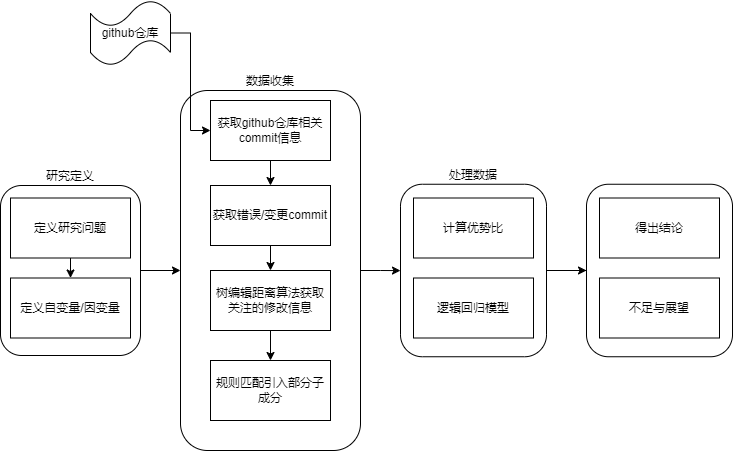
\includegraphics[width=0.8\textwidth]{picture/study_process.png}
  \caption{研究流程}
  \label{fig:image1}
\end{figure}

\section{研究仓库选取}  
这项研究的依据是十二个Rust系统的变更历史和问题跟踪系统。egui是一个用Rust编写的简单、快速、可移植的GUI库,主要用于开发即时模式的用户界面。它不依赖于本地操作系统提供的UI组件,因此可以轻松集成到各种应用程序中。iced是一个跨平台的GUI库,灵感来自于Elm语言的架构。它旨在创建纯Rust开发的简洁、反应灵敏的GUI应用程序,支持异步编程。nushell(通常称为nu)是一个新型的命令行shell,用Rust编写,结合了传统的shell功能和现代的数据处理能力。它支持表格数据的原生处理,使得对JSON、YAML等数据的处理更为直观和强大。clap是一个用于解析命令行参数和配置的库。它功能丰富,易于使用,支持自动生成帮助信息和错误消息,是创建命令行应用程序的理想选择。starship是一个快速、可定制的shell提示符,适用于多种shell(如bash、zsh、fish等)。它可以显示各种有用的信息,比如Git分支、Rust版本等,并且外观和功能高度可定制。TiKV是一个分布式键值数据库,最初由PingCAP公司开发,用于支持TiDB数据库的事务层。TiKV支持事务,提供强一致性保证,并通过Raft协议\cite{ongaro2014search}实现多副本数据复制。Firecracker是由Amazon Web Services开发的开源虚拟化技术,专为运行微虚拟机(microVMs)而设计,支持安全、高效地运行云原生服务器less计算工作负载。Tokio是一个Rust异步运行时,基于Rust的异步编程特性,广泛用于高性能网络服务和应用程序的开发。它支持异步I/O、任务调度等功能。Diem(前称Libra)是由Facebook启动的一个区块链项目,旨在创建一个稳定、无国界的数字货币。项目的目的是提供一种更安全、更低成本的支付方式。Vaultwarden是一个轻量级的Bitwarden密码管理服务的开源实现。它允许用户自行托管自己的密码库,而无需依赖第三方服务。actix-web是一个功能强大、易于使用的异步Web框架,支持构建高性能的Web应用程序。它基于Actix actor框架和Tokio异步运行时。rome/tools 是 Rome 的工具集,主要用于前端开发,包括代码格式化、linting、打包等功能。Rome 旨在成为一个全面的前端工具链,使前端开发更加统一和高效。

我们选取上述仓库的原因有如下几点:
\begin{enumerate}
    \item 这些仓库都是用 Rust 编程语言编写的,体现出了 Rust 在多种领域内的实际应用,包括 GUI 开发、命令行工具、网络编程、虚拟化技术、分布式系统等各种领域。
    \item 这些仓库都是在github中十分活跃,拥有很高的star数,受rust开发者广泛关注。
    \item 这些仓库的开发严格遵守开发规范,如pr、merge等行为有严格的规范,这样可以提高我们统计的准确性,减少因为开发者不规范导致的噪声。
\end{enumerate}

我们通过上述的仓库,采用预先设计的方法,进行实验数据的获取,并对获取实验数据进行分析,得到实验结论,并针对实验结论进行一定的分析。

以错误倾向为例,我们首先使用python脚本进行仓库的获取,然后从仓库的issue中找出特定标签的commit,通过我们设计的定义,找出引入这些错误的commit,使用工具获取这些commit中新引入的语法项以及语法项具体子成分,与其他非引入错误的commit进行对比,获得实验结论并对其分析讨论。

另外,我们在这里给出仓库的一些基本信息。

表\ref{tab:repo-info}给出了仓库的一些基本信息,commit表示仓库中commit的数量,Issue表示仓库主页issue的数目,GitHub Issue 是 GitHub 项目中用于追踪和讨论项目相关问题的功能。它可以被用来报告 bug、请求新功能、或者提出项目中的其他任务和问题。
\begin{table}[ht]
	\centering
        \caption{研究仓库信息}
	\begin{tabular}{ccccc}
        \toprule
		\textbf{repos}                             & \textbf{commit(个)} & \textbf{issue(个)} & \textbf{code line(行)} & \textbf{文件个数(个)} \\
        \midrule
		tikv/tikv                         & 7499   & 3567  & 446921    & 1183     \\
		nushell/nushell                   & 7994   & 3527  & 178342    & 1127     \\
		rome/tools                        & 4309   & 1353  & 247459    & 1262     \\
		iced-rs/iced                      & 3923   & 695   & 45819     & 323      \\
		  actix/actix-web                 & 4467   & 1389  & 52536     & 286      \\
		  firecracker-microvm/firecracker & 5898   & 1294  & 67816     & 276      \\
		  dani-garcia/vaultwarden         & 2649   & 1904  & 21301     & 52       \\
		  diem/diem                       & 9840   & 1060  & 323752    & 1730     \\
		tokio-rs/tokio                  & 3603   & 1801  & 79468     & 693      \\
		  clap-rs/clap                    & 7761   & 1671  & 52983     & 330      \\
		emilk/egui                        & 2754   & 861   & 56286     & 231      \\
		starship/starship                 & 2973   & 1501  & 35054     & 204  \\
        \bottomrule
	\end{tabular}
	\label{tab:repo-info}
\end{table}

表\ref{tab:bug-introduce-info}介绍了错误引入相关研究的信息,由于Rust版本变更十分漫长,过于旧的版本,不再具备参考价值,所以我们选取的是各仓库2021年之后的commit信息。

\begin{table}[ht]
	\centering
        \caption{错误引入信息}
	\begin{tabular}{ccc}
        \toprule
		\textbf{repos}                             & \textbf{错误引入commit(个)} & \textbf{非错误引入commit(个)} \\
        \midrule
		tikv/tikv                         & 649        & 1385        \\
		nushell/nushell                   & 704        & 4411        \\
		rome/tools                        & 334        & 1966        \\
		iced-rs/iced                      & 70         & 2278        \\
		  actix/actix-web                 & 50         & 891         \\
		  firecracker-microvm/firecracker & 18         & 2632        \\
		  dani-garcia/vaultwarden         & 42         & 1169        \\
		  diem/diem                       & 19         & 2430        \\
		tokio-rs/tokio                    & 126        & 1169        \\
		  alacritty/alacritty             & 98         & 425         \\
		  clap-rs/clap                    & 136        & 3811        \\
		emilk/egui                        & 250        & 1646        \\
		starship/starship                 & 106        & 1620 \\
        \bottomrule
	\end{tabular}
	\label{tab:bug-introduce-info}
\end{table}

\section{研究定义}
\subsection{研究问题}
为了研究Rust 语法结构与变更及错误倾向性的关系,我们设计了如下几个研究问题,试图通过下面的问题来得到一定的结论,这些问题由浅入深地研究了我们的研究主题。
\begin{itemize}
    \item RQ1: 不同语法项与变更倾向性之间的关系是什么?在这里我们研究各种语法项是不是容易发生变更,不同语法项之间会不会有哪些更容易发生变更。
    - H01: 某些语法项比其他语法项更易变更。
    \item RQ2: 特定语法项中的引入类型与变更倾向性之间的关系是什么?我们进一步观察每个语法项内部的各个子成分对于变更倾向的影响。
    - H02: 某种语法结构中的特定引入类型比其他类型更易变更。
    \item RQ3: 不同语法项与错误倾向性之间的关系是什么?在这里我们研究各种语法项是不是容易引入错误,不同语法项之间会不会有哪些明显更容易引发错误。
    - H03: 某些语法项比其他语法项更易出现错误。
    \item RQ4: 特定语法项中的引入类型与错误倾向性之间的关系是什么?我们进一步观察每个语法项内部的各个子成分对于引入错误的影响。
      - H04: 某种语法结构中的特定引入类型比其他类型更易出现错误。
\end{itemize}

\subsection{自变量}
Rust Reference 是 Rust 编程语言的官方参考手册,它提供了详尽的说明和解释,涵盖 Rust 语言的所有语法和特性。在我们的实验中,我们从该参考手册选取了items作为研究对象:

\begin{itemize}
    \item Module (mod): 用于组织代码,将功能相关的代码块分组在一起。模块可以嵌套,有助于创建清晰的代码结构。
    \item ExternCrate: 在2018 edition之前,用于声明外部库的依赖关系。在Rust 2018 edition中,这一语法项通常不再需要,因为Cargo.toml文件已足够处理外部依赖。
    \item ConstantItem (const): 用于定义常量,这些常量在编译时就已确定值,且值不可变。
    \item MacroInvocationSemi: 指在代码中调用宏时用分号结尾的语法结构,常用于执行宏而不返回值。
    \item MacroRulesDefinition (macro\_rules!): 定义宏的语法结构,允许编写可重复使用的代码模式。
    \item ExternBlock (extern): 用于声明外部函数接口,常用于与C语言等其他语言的互操作。
    \item Struct: 定义一个结构体,用于创建带有多个可能不同类型的字段的数据类型。
    \item Union: 类似结构体,但所有字段共享内存。常用于底层系统编程中的内存节省和特定类型操作。
    \item Enumeration (enum): 用于定义一个可以是几种不同值中的一个的类型。
    \item TypeAlias (type): 用于给现有的类型创建别名,有助于简化复杂类型的使用或提高代码的可读性。
    \item Function (fn): 定义一个函数,是执行代码的基本单元。
    \item Implementation (impl): 用于给结构体、枚举或特性实现具体的方法和关联函数。
    \item Trait: 定义一组方法(可以包含实现),其他类型可以实现(impl)这些方法,实现接口编程。
    \item AssociatedType: 在trait定义内部定义的类型,使得trait可以在不同的实现中具有不同的类型。
    \item UseDeclaration (use): 用于引入作用域中的路径,简化类型或函数的访问。
    \item StaticItem (static): 定义全局变量,这些变量在程序运行期间始终存在,与const的不同之处在于,static可以是可变的。
    \item GenericParams: 在定义函数、结构体、枚举、trait时,使用泛型参数使其可以适用于多种数据类型。
\end{itemize}
对于各语法项,我们选取了我们关注的一些语法成分,试图用模型衡量它们对于变更或错误引入倾向性的影响。下面是我们为各个语法项选取的子成分。
\begin{table}[tbp]
	\centering
        \caption{各个语法项关注的子成分}
	\begin{tabular}{cccccc}
        \toprule
		\textbf{语法项}            & \textbf{子成分1}                & \textbf{子成分2}         & \textbf{子成分3}         & \textbf{子成分4}         & \textbf{子成分5}        \\
        \midrule
		ExternCrate    & CrateRef            & AsClause     &              &              &             \\
		ConstantItem   & type                & expression   &              &              &             \\
		ExternBlock    & unsafe              & Abi          & Visibility   &              &             \\
		Struct         & visibility\_modifier & type         &              &              &             \\
		Union          & visibility\_modifier & type         &              &              &             \\
		Enumeration    & visibility\_modifier & expression   & type         &              &             \\
		TypeAlias      & lifetime            & trait\_bounds &              &              &             \\
		Function       & function\_modifiers  & parameters   & lifetime     & trait\_bounds & return\_type \\
		Implementation & unsafe              & lifetime     & trait\_bounds & TypePath     &             \\
		Trait          & unsafe              & lifetime     & trait\_bounds &              &             \\
		StaticItem     & mut                 & type         & expression   &              &             \\
		GenericParams  & LifetimeParam       & ConstParam   & TypeParam    &              &          \\
        \bottomrule
	\end{tabular}
	\label{tab:components}
\end{table}

如表2-1,我们展示了在探讨语法项子成分对变更和错误倾向性的影响时我们所关注的语法项的子成分。在这里,我们介绍一下我们关注他们的理由。
\begin{itemize}
    \item ExternCrate(CrateRef, AsClause): 我们关注CrateRef因为它直接指向外部库的引用,这是理解依赖管理的关键;而AsClause则使我们能够观察到命名空间的自定义使用,影响代码的可读性和可维护性。
    \item ConstantItem(type, expression): 我们关注type是因为它定义了常量的数据类型,直接影响程序的类型安全;expression则体现了常量的计算逻辑,可能是错误和性能问题的源头。
    \item ExternBlock(unsafe, Abi, Visibility): 我们关注unsafe以理解潜在的安全风险点;Abi指明了与外部代码的接口,关键于跨语言调用的稳定性;Visibility决定了访问级别,影响模块之间的耦合度。
    \item Struct(visibility\_modifier, type): 我们关注visibility\_modifier来分析结构体的可访问性,这直接影响模块的封装性;type则定义了结构体的数据类型,是理解数据组织的基础。
    \item Enumeration(visibility\_modifier, expression, type): 我们关注visibility\_modifier以审视枚举的公开级别;expression和type则共同定义了枚举的值和类型,关键于程序的逻辑分支处理。
    \item TypeAlias(lifetime, trait\_bounds): 我们关注lifetime以评估类型别名在生命周期管理中的作用;trait\_bounds则揭示了类型约束,对理解类型的行为和兼容性至关重要。
    \item Function(function\_modifiers, parameters, lifetime, trait\_bounds, return\_type): 我们关注function\_modifiers来了解函数的特殊属性如异步或不可变性;parameters, lifetime, trait\_bounds, 和return\_type共同定义了函数的接口和行为,是理解函数设计和使用的核心。
    \item Implementation(unsafe, lifetime, trait\_bounds, TypePath): 我们关注unsafe因为它表明代码中潜在的高风险区域;lifetime和trait\_bounds提供了实现细节的上下文,而TypePath则定位具体实现的结构或特性。
    \item Trait(unsafe, lifetime, trait\_bounds): 我们关注unsafe以识别特性中的安全漏洞;lifetime和trait\_bounds则是理解特性的行为限制和扩展性的关键。
    \item StaticItem(mut, type, expression): 我们关注mut以监控全局变量的可变性,这对并发编程至关重要;type和expression则分别定义了静态项的数据类型和初始化逻辑,直接关联到程序的运行时状态。
    \item GenericParams(LifetimeParam, ConstParam, TypeParam): 我们关注LifetimeParam以评估泛型在生命周期管理中的角色;ConstParam和TypeParam则分别揭示了泛型参数的常量性质和类型多样性,是泛型编程的基石。
\end{itemize}

对于RQ1和RQ3,我们统计每个commit中新增部分所属的item,定义为$A_{ic}$ commit $c$ 中统计到的item $i$ 的数量。对于RQ2和RQ4,我们统计到具体item下具体的子成分,定义$A{ijc}$ 为commit $c$ 中统计到的item $i$ 中的子成分 $j$ 的数量。

\subsection{因变量}
\label{sec:dependent-var}
因变量对应不同item或其子成分影响下commit发生的现象。

RQ1和RQ2 变更倾向指的是在一个commit中的所有文件中,是否存在某个文件发生了变更。变更被定义为从已有的代码变为新的代码,对应增删查改中的改。在进行源代码变更分析中,使用 tree-sitter-rust 来生成 Rust 语言的抽象语法树(AST)是研究的关键一环。tree-sitter-rust 是 tree-sitter 的一个针对 Rust 语言定制的模块,专门设计以解析 Rust 代码并生成遵循 Rust 语法规则的 AST。这一特性使得能够在语法层面上精确地分析代码变更,例如识别特定的语法结构在不同版本代码中的修改或替换。

通过比较连续两次提交的 AST 差异,本研究能够精确识别代码中的具体修改,并进一步分析这些修改对软件质量和功能的影响。

RQ3和RQ4 
在我的研究中,错误倾向性被定义为在代码提交(commit)过程中新引入部分倾向于引入错误。对于引入错误的代码,我们试图实现自动化的识别方法,我们认为错误的引入可以从错误的修复来获取,修复错误的部分必定与引入错误的部分有关联,基于这个思想,我们有了错误引入的定义:对于一个commit,如果存在后来修复错误的commit修改了它引入的部分,则认为该commit发生了错误引入。

\section{数据收集}
我们的研究主题是RUST语法结构与变更及错误倾向性关系,要想研究二者关系,首先要获取到语法结构与变更或错误对应的变量,在前一节我们已经给出了相关变量的定义。在这里,我们的工作重点就在于如何收集这些数据,下面我们介绍数据收集的各个环节。

\begin{minipage}{\textwidth}
\begin{parcolumns}{2}
\colchunk{
\floatname{listing}{代码示例}
\begin{lstlisting}[caption={简单的求和程序}, keepspaces=true, label={code1}]
// version1
fn sum(nums: &[i32])->i32 {
  let mut total = 0;
  for num in nums {
      total += num;
  }
  total
}

fn main() {
  let data = vec![1, 2];
  print!("{}", sum(&data));
} 
\end{lstlisting}
}

\colchunk{
\begin{lstlisting}[caption={简化过的求和程序}, keepspaces=true, label={code2}]
// version2
fn sum(nums: &[i32])->i32 {
  nums.iter().sum()
}

fn main() {
  let data = vec![1, 2, 3];
  print!("{}", sum(&data));
}
\end{lstlisting}
}

\colplacechunks
\end{parcolumns}
\end{minipage}

\subsection{收集错误修复commit}
我们实现了自动化的获取脚本,具体工作细节如下:首先定义github仓库以及各仓库相关的标签列表,借助github api从github根据标签爬取相关的commit hash,根据commit hash 获取每次commit中改动的后缀为.rs的文件,存放在文件中,再根据commit hash和文件名将文件前后的变更保存到一个目录中。

\subsection{获取每次commit新增部分}
\textit{difftastic}\footnote{\url{https://github.com/Wilfred/difftastic}} 工具是一个开源的源代码比较工具,与简单的文本比对不同,它借用tree-sitter将源代码解析为语法树,紧接着对语法树进行树编辑距离算法(核心是dijkstra算法)\cite{bille2005survey, pawlik2011rted, demaine2007optimal},得出前后改动的内容,这样的从语法层面的前后比较,比传统的文本比对更加精确,更加符合我们的需求。我们借用difftastic输出的中间结果,生成一个存放Hunk的向量,它代表左右子树各自新的内容,右子树新的内容即为我们关注的新增部分,如上面\ref{code1}和\ref{code2}代码段,version2中1,3,7,8行是新增行,他们要么是在version1中找不到相同的行(比如第一行注释行),要么有了新的修改(比如第7行的vec声明中多了一个元素)。

\subsection{获取每次commit删除部分}
同新增部分,我们借用difftastic输出的中间结果,生成一个存放Hunk的向量,左子树Hunk对应的内容,即删除部分。如上面\ref{code1}和\ref{code2}代码段,version1中的2,3,4,5,6行在version2中找不到相同的代码行,我们认为2,3,4,5,6行是被删除的行。

\subsection{收集错误引入commit}
为了准确地测量这种倾向性,我采用了一种基于历史数据的方法,通过分析开源项目的issue追踪系统中的标签来识别错误修复的提交(commit)。在算法\ref{algorithm1}中,我们简单描述了这个过程。具体来说,首先我们需要上面获取到的错误修复commit。一旦一个commit被标记为错误修复commit,将其标记为commit C。

为了确定哪些先前的提交可能引入了这些错误,我遍历了每个错误修复commit之前的所有普通commit。通过比较这些普通commit和commit C的代码变更部分,如果发现普通commit中的代码修改与commit C有交集,即这些修改出现在后来的错误修复提交中,那么这些普通commit被标记为错误引入commit。这种方法允许我们直接关联特定的代码修改与后续修复的错误,从而揭示代码变更的质量和风险。

此处我们简化了算法,在实际收集信息时,每个commit的情况会非常复杂,我们需要基于一定的策略过滤掉无关commit,过滤掉无关文件。对于每个commit而言,它们往往不止有一个文件,在上面的算法中我们均假设只有一个文件,但多文件也只是增加了写代码的难度,基本策略都是一致的。

我使用了tree-sitter-rust来生成Rust代码的抽象语法树(AST),从而在更细粒度上比较代码变更。通过AST,可以更精确地识别和分析哪些具体的语法结构变更可能与错误的引入有关。这种基于AST的分析方法不仅提高了识别错误倾向的准确性,也增强了对代码变更影响的理解。

在实际操作中,我对多个开源Rust项目的历史提交数据进行了此类分析。这包括从项目的Git仓库中提取所有commit记录,然后使用自动化脚本标记含有错误的commit,并追溯可能引入错误的普通commit。通过这种方法,我能够收集到大量数据,这些数据不仅支持了对错误引入模式的深入分析,也为理解编码实践中的常见问题提供了实证基础。

\begin{algorithm}
\caption{搜索错误引入commit}
\label{algorithm1}
\begin{algorithmic}[1]
\State $\text{commit\_map} \gets \text{HashMap<Commit, Set<Commit>>}$
\ForAll{$C \in \text{Commits}$}
    \State $B0, B0' \gets \text{parse}(C)$
    \ForAll{$C' \in \text{Commits before } C$}
        \State $B1, B1' \gets \text{parse}(C')$
        \State $A \gets \text{get_addition}(B1, B1')$
        \State $D \gets \text{get_deletion}(B0, B0')$
        \State $res \gets \text{has\_intersection}(B1', B0, A, D)$
        \If{$res = 1$}
            \State $\text{commit\_map.add}(C, C')$
        \EndIf
    \EndFor
\EndFor
\State \Return $\text{commit\_map}$
\end{algorithmic}
\end{algorithm}

\subsection{获取新引入item以及其组成部分}
通过difftastic工具获取新引入的tree-sitter语法树节点,这个节点一般是叶子结点,即表示源代码中具体某个token的节点,比如函数中的fn、int32类型、funcname。我们找到该节点,然后在语法树中从叶子结点到根节点向上搜索,选取第一个遇到的item为新引入item,如果该item是另一个item的子节点,只选取最近的祖先item作为新引入节点。通过编写预定的规则,去匹配目标的component,编写的算法可以匹配大部分情况,准确性很高。

如算法\ref{algorithm2}所示,我们首先定义一个遍历栈,从叶子结点开始向根节点遍历,每次把途经节点加入到遍历栈中,一旦我们的遍历找到类型为语法项的节点,我们停止遍历,此时栈中的内容即为语法项到具体改动叶子节点的路径,我们通过将此路径与预先定义的规则相匹配,即可找到本次item改动的具体类型。其中,ITEM2COMPONENTS是我们定义的一个哈希表,它的键是语法树节点,值是可能存在我们所关注子成分的子节点,这样我们从语法项节点向叶子节点的方向进行搜索,每次查询当前节点是否在父亲节点关注的子节点中,如果在,则继续遍历;如果发现不在,则说明后面的内容没有我们所关注的子节点。

\begin{algorithm}
\caption{获取语法项对应组件的函数}
\label{algorithm2}
\begin{algorithmic}[1]
\Function{GetComponentOfItemNode}{$\text{cursor1}: \text{TreeCursor}$}
    \State $\text{cursor} \gets \text{clone}(\text{cursor1})$
    \State $\text{travel\_stack} \gets \text{empty stack}$
    \State $\text{item\_string} \gets \text{empty string}$
    \While{$\text{not at root}$}
        \If{$\text{cursor node is syntax item}$}
            \State $\text{item\_string} \gets \text{cursor node kind}$
            \State $\textbf{break}$
        \EndIf
        \State $\text{push cursor node to travel\_stack}$
        \State $\text{move cursor to parent}$
    \EndWhile
    \State $\text{map} \gets \text{ITEM2COMPONENTS[item\_string]}$
    \For{$\text{node} \gets \text{travel\_stack.reverse()}$}
        \If{$\text{map contains key(node.kind)}$}
            \If{$\text{map[node.kind].kind} == \text{ChilditemKind::Container}$}
                \State $\text{map} \gets \text{ITEM2COMPONENTS[node.kind]}$
            \Else
                \State \Return $\text{node}, \text{map[node.kind].name}$
            \EndIf
        \Else
            \State \Return $\text{None}$
        \EndIf
    \EndFor
    \State \Return $\text{None}$
\EndFunction
\end{algorithmic}
\end{algorithm}

\section{数据分析}
RQ1和RQ3:我们为了研究commit中的变更和错误引入是否跟某些语法item的引入有关,我们计算了优势比(odds ratio\cite{bland2000odds}),他表示一个事件发生的可能性,比如说变更,OR被定义为一个样本中事件发生的几率p与另一个样本中发生的几率q的比值:OR = p/(1-p) / q/(1-q)。比值比为1表示两个样本中事件发生的可能性相同。OR > 1 表示事件在第一个样本中(含有某些语法item的实验组commit)更有可能发生,而OR < 1 表示相反的情况(不含有某些语法item的对照组commit)。

RQ2和RQ4:逻辑回归可以用于进行影响力分析,尤其是当你想了解哪些变量对某个具体事件(通常是二元的)的发生有显著影响时。我们为了研究语法item的特定子成分变更与错误和变更之间的关系,在这里使用逻辑回归模型进行一个统计分析,统计特定语法item的各种子成分对于变更/引入错误是否有显著影响。\cite{stoltzfus2011logistic}

在逻辑回归模型中,因变量通常是二元变量,因此它假定两个值{0,1},例如,变更与否。多变量逻辑回归基于如下的公式:

$π(X1, X2, ..., Xn) = \frac{e^{C0+C1·X1+...+Cn·Xn}} { 1 + e^{C0+C1·X1+...+Cn·Xn}}$

\begin{itemize}
    \item Xi是描述被建模现象的特征,在我们的案例中是参与第i种变更类型的item的数量。
    \item 0 ≤ π ≤ 1是逻辑回归曲线上的一个值。这个值越接近1表示发生变更的概率越高。
\end{itemize}

\chapter{研究结果}
通过实验,我们获得了一定的研究结果数据,我们在本章展示这些结果数据,给出由结果数据得出的结论,并对结论结合我们对于仓库具体变更情况的观察,分析所得结论的原因。

在问题一和三的表格中,表格中值为OR/p-value;在问题二和四的表格中,表格中值为C/p-value。另外,表格颜色为橙色表示数据呈负(抑制)作用,绿色表示数据呈正(促进)作用,灰色表示数据无效。

\section{结果一:不同语法项与变更倾向性之间的关系}

\begin{table}[ht]
	\centering
	\caption{RQ1研究结果a}
	\begin{tabular}{cccccc}
        \toprule
		\textbf{repo}        & \textbf{领域}          & \textbf{Module}    & \textbf{ExternCrate} & \textbf{ConstantItem} & \textbf{MacroInvocationSemi} \\
        \midrule
		egui        & GUI框架       & \cellcolor{orange!30}0.33/0.0  & \cellcolor{gray!20}nan/1.0     & \cellcolor{gray!20}1.057/0.723  & \cellcolor{orange!30}0.621/0.0           \\
		iced        & GUI框架       & \cellcolor{orange!30}0.109/0.0 & \cellcolor{gray!20}nan/1.0     & \cellcolor{gray!20}0.362/0.0    & \cellcolor{orange!30}0.485/0.0           \\
		nushell     & 命令行工具与Shell & \cellcolor{orange!30}0.074/0.0 & \cellcolor{gray!20}0.0/0.126   & \cellcolor{gray!20}0.451/0.0    & \cellcolor{orange!30}0.466/0.0           \\
		clap        & 命令行工具与Shell & \cellcolor{orange!30}0.156/0.0 & \cellcolor{gray!20}nan/1.0     & \cellcolor{green!20}1.45/0.006   & \cellcolor{orange!30}0.822/0.0           \\
		starship    & 命令行工具与Shell & \cellcolor{orange!30}0.022/0.0 & \cellcolor{gray!20}0.0/0.502   & \cellcolor{orange!30}0.101/0.0    & \cellcolor{orange!30}0.781/0.026         \\
		tikv        & 系统编程与虚拟化    & \cellcolor{orange!30}0.1/0.0   & \cellcolor{orange!30}0.191/0.0   & \cellcolor{orange!30}0.341/0.0    & \cellcolor{orange!30}0.332/0.0           \\
		firecracker & 系统编程与虚拟化    & \cellcolor{orange!30}0.13/0.0  & \cellcolor{gray!20}nan/1.0     & \cellcolor{orange!30}0.764/0.022  & \cellcolor{orange!30}0.637/0.0           \\
		tools       & 开发工具 & \cellcolor{orange!30}0.064/0.0 & \cellcolor{gray!20}nan/1.0     & \cellcolor{orange!30}0.643/0.0    & \cellcolor{orange!30}0.484/0.0           \\
		tokio       & 异步运行时       & \cellcolor{orange!30}0.195/0.0 & \cellcolor{gray!20}0.0/1.0     & \cellcolor{orange!30}0.454/0.0    & \cellcolor{orange!30}0.851/0.024         \\
		diem        & 区块链和安全      & \cellcolor{orange!30}0.151/0.0 & \cellcolor{gray!20}0.0/0.476   & \cellcolor{orange!30}0.409/0.0    & \cellcolor{orange!30}0.615/0.0           \\
		vaultwarden & 区块链和安全      & \cellcolor{orange!30}0.071/0.0 & \cellcolor{gray!20}inf/0.125   & \cellcolor{orange!30}0.587/0.006  & \cellcolor{orange!30}0.445/0.0           \\
		actix-web   & 网络框架        & \cellcolor{orange!30}0.187/0.0 & \cellcolor{gray!20}0.642/0.305 & \cellcolor{orange!30}0.557/0.026  & \cellcolor{orange!30}0.801/0.013   \\
        \bottomrule
	\end{tabular}
	\label{tab:RQ1-1}
\end{table}

由表\ref{tab:RQ1-1}可以得出结论:Module、ConstantItem、MacroInvocationSemi不容易发生变更;ExternCrate无法得出有效结论。

\begin{table}[ht]
	\centering
	\caption{RQ1研究结果b}
	\begin{tabular}{ccccc}
        \toprule
		\textbf{repo}        & \textbf{领域}          & \textbf{MacroRulesDefinition} & \textbf{ExternBlock} & \textbf{Struct}      \\
        \midrule
		egui        & GUI框架       & \cellcolor{orange!30}0.237/0.0            & \cellcolor{gray!20}0.511/0.483 & \cellcolor{orange!30}0.607/0.0   \\
		iced        & GUI框架       & \cellcolor{gray!20}2.459/0.059          & \cellcolor{gray!20}nan/1.0     & \cellcolor{orange!30}0.885/0.039 \\
		nushell     & 命令行工具与Shell & \cellcolor{orange!30}0.586/0.015          & \cellcolor{gray!20}nan/1.0     & \cellcolor{orange!30}0.621/0.0   \\
		clap        & 命令行工具与Shell & \cellcolor{gray!20}0.997/1.0            & \cellcolor{gray!20}nan/1.0     & \cellcolor{orange!30}0.868/0.025 \\
		starship    & 命令行工具与Shell & \cellcolor{green!20}4.637/0.048          & \cellcolor{gray!20}nan/1.0     & \cellcolor{orange!30}0.126/0.0   \\
		tikv        & 系统编程与虚拟化    & \cellcolor{gray!20}0.836/0.074          & \cellcolor{gray!20}0.0/1.0     & \cellcolor{orange!30}0.526/0.0   \\
		firecracker & 系统编程与虚拟化    & \cellcolor{gray!20}0.761/0.209          & \cellcolor{gray!20}nan/1.0     & \cellcolor{orange!30}0.66/0.0    \\
		tools       & 开发工具 & \cellcolor{orange!30}0.511/0.0            & \cellcolor{gray!20}0.245/0.214 & \cellcolor{orange!30}0.547/0.0   \\
		tokio       & 异步运行时       & \cellcolor{orange!30}0.674/0.008          & \cellcolor{gray!20}nan/1.0     & \cellcolor{orange!30}0.684/0.0   \\
		diem        & 区块链和安全      & \cellcolor{green!20}1.753/0.008          & \cellcolor{gray!20}nan/1.0     & \cellcolor{orange!30}0.73/0.0    \\
		vaultwarden & 区块链和安全      & \cellcolor{gray!20}0.784/0.153          & \cellcolor{gray!20}nan/1.0     & \cellcolor{orange!30}0.168/0.0   \\
		actix-web   & 网络框架        & \cellcolor{green!20}2.294/0.0            & \cellcolor{gray!20}nan/1.0     & \cellcolor{gray!20}0.912/0.393   \\
        \bottomrule
	\end{tabular}
	\label{tab:RQ1-2}
\end{table}

由表\ref{tab:RQ1-2}可以得出:Struct不容易发生变更,MacroRulesDefinition、ExternBlock无法得出有效结论。

\begin{table}[ht]
	\centering
	\caption{RQ1研究结果c}
	\begin{tabular}{cccccc}
        \toprule
		\textbf{repo}        & \textbf{领域}          & \textbf{Enumeration} & \textbf{TypeAlias}   & \textbf{Function}    & \textbf{Implementation} \\
        \midrule
		egui        & GUI框架       & \cellcolor{orange!30}0.487/0.0   & \cellcolor{orange!30}0.59/0.002  & \cellcolor{green!20}1.35/0.0    & \cellcolor{orange!30}0.275/0.0      \\
		iced        & GUI框架       & \cellcolor{orange!30}0.56/0.0    & \cellcolor{orange!30}0.318/0.0   & \cellcolor{green!20}1.42/0.0    & \cellcolor{orange!30}0.487/0.0      \\
		nushell     & 命令行工具与Shell & \cellcolor{orange!30}0.417/0.0   & \cellcolor{orange!30}0.533/0.0   & \cellcolor{gray!20}0.932/0.134 & \cellcolor{orange!30}0.387/0.0      \\
		clap        & 命令行工具与Shell & \cellcolor{orange!30}0.461/0.0   & \cellcolor{orange!30}0.204/0.0   & \cellcolor{gray!20}0.914/0.091 & \cellcolor{orange!30}0.57/0.0       \\
		starship    & 命令行工具与Shell & \cellcolor{orange!30}0.282/0.0   & \cellcolor{gray!20}0.571/0.399 & \cellcolor{green!20}1.559/0.016 & \cellcolor{orange!30}0.259/0.0      \\
		tikv        & 系统编程与虚拟化    & \cellcolor{orange!30}0.346/0.0   & \cellcolor{orange!30}0.655/0.0   & \cellcolor{orange!30}0.574/0.0   & \cellcolor{orange!30}0.262/0.0      \\
		firecracker & 系统编程与虚拟化    & \cellcolor{orange!30}0.472/0.0   & \cellcolor{orange!30}0.453/0.0   & \cellcolor{green!20}1.461/0.0   & \cellcolor{orange!30}0.358/0.0      \\
		tools       & 开发工具 & \cellcolor{orange!30}0.456/0.0   & \cellcolor{orange!30}0.586/0.0   & \cellcolor{green!20}1.107/0.11  & \cellcolor{orange!30}0.343/0.0      \\
		tokio       & 异步运行时       & \cellcolor{orange!30}0.608/0.023 & \cellcolor{orange!30}0.455/0.0   & \cellcolor{green!20}1.132/0.008 & \cellcolor{orange!30}0.289/0.0      \\
		diem        & 区块链和安全      & \cellcolor{orange!30}0.499/0.0   & \cellcolor{orange!30}0.547/0.0   & \cellcolor{green!20}1.241/0.041 & \cellcolor{orange!30}0.345/0.0      \\
		vaultwarden & 区块链和安全      & \cellcolor{orange!30}0.071/0.0   & \cellcolor{orange!30}0.23/0.0    & \cellcolor{orange!30}0.451/0.0   & \cellcolor{orange!30}0.156/0.0      \\
		actix-web   & 网络框架        & \cellcolor{green!20}1.681/0.0   & \cellcolor{gray!20}1.098/0.563 & \cellcolor{green!20}1.427/0.0   & \cellcolor{orange!30}0.573/0.0   \\
        \bottomrule     
	\end{tabular}
	\label{tab:RQ1-3}
\end{table}

由表\ref{tab:RQ1-3}可以得出:Enumeration、TypeAlias、Implementation不容易发生变更,Function较多数据表现出变更倾向。

\begin{table}[ht]
	\centering
	\caption{RQ1研究结果d}
	\begin{tabular}{cccccc}
        \toprule
		\textbf{repo}        & \textbf{领域}          & \textbf{Trait}       & \textbf{StaticItem}  & \textbf{UseDeclaration} & \textbf{GenericParams} \\
        \midrule
		egui        & GUI框架       & \cellcolor{gray!20}0.738/0.077 & \cellcolor{gray!20}0.853/1.0   & \cellcolor{gray!20}1.043/0.535    & \cellcolor{orange!30}0.467/0.0     \\
		iced        & GUI框架       & \cellcolor{orange!30}0.32/0.0    & \cellcolor{gray!20}1.212/0.618 & \cellcolor{orange!30}0.709/0.0      & \cellcolor{orange!30}0.584/0.0     \\
		nushell     & 命令行工具与Shell & \cellcolor{gray!20}1.133/0.624 & \cellcolor{orange!30}0.426/0.026 & \cellcolor{orange!30}0.883/0.0      & \cellcolor{orange!30}0.41/0.0      \\
		clap        & 命令行工具与Shell & \cellcolor{gray!20}1.227/0.133 & \cellcolor{green!20}2.626/0.0   & \cellcolor{orange!30}0.621/0.0      & \cellcolor{orange!30}0.545/0.0     \\
		starship    & 命令行工具与Shell & \cellcolor{orange!30}0.0/0.033   & \cellcolor{gray!20}0.573/0.691 & \cellcolor{gray!20}0.873/0.308    & \cellcolor{orange!30}0.605/0.035   \\
		tikv        & 系统编程与虚拟化    & \cellcolor{orange!30}0.385/0.0   & \cellcolor{orange!30}0.06/0.0    & \cellcolor{green!20}1.456/0.0      & \cellcolor{orange!30}0.531/0.0     \\
		firecracker & 系统编程与虚拟化    & \cellcolor{orange!30}0.178/0.0   & \cellcolor{gray!20}1.184/0.727 & \cellcolor{orange!30}0.762/0.0      & \cellcolor{orange!30}0.556/0.001   \\
		tools       & 开发工具 & \cellcolor{orange!30}0.537/0.0   & \cellcolor{gray!20}1.051/1.0   & \cellcolor{green!20}1.618/0.0      & \cellcolor{orange!30}0.512/0.0     \\
		tokio       & 异步运行时       & \cellcolor{orange!30}0.538/0.008 & \cellcolor{gray!20}1.217/0.713 & \cellcolor{orange!30}0.745/0.0      & \cellcolor{orange!30}0.324/0.0     \\
		diem        & 区块链和安全      & \cellcolor{orange!30}0.528/0.0   & \cellcolor{orange!30}0.716/0.017 & \cellcolor{green!20}1.338/0.0      & \cellcolor{orange!30}0.578/0.0     \\
		vaultwarden & 区块链和安全      & \cellcolor{gray!20}nan/1.0     & \cellcolor{orange!30}0.315/0.0   & \cellcolor{gray!20}1.052/0.565    & \cellcolor{orange!30}0.364/0.0     \\
		actix-web   & 网络框架        & \cellcolor{gray!20}0.855/0.412 & \cellcolor{gray!20}0.669/0.284 & \cellcolor{gray!20}1.055/0.547    & \cellcolor{orange!30}0.751/0.025   \\
        \bottomrule  
	\end{tabular}
	\label{tab:RQ1-4}
\end{table}

由表\ref{tab:RQ1-4}可以得出:GenericParams不容易发生变更,Trait、StaticItem、UseDeclaration无法得出结论。


综上,研究问题一可以得出如下的结论:

\begin{enumerate}
    \item Function 展现出相对较高的变更倾向。
    \item ExternCrate、MacroRulesDefinition、UseDeclaration、Trait、ExternBlock 和 StaticItem的数据量较少或异常,难以得出明确结论。
    \item Module、Constantitem、Enumeration,TypeAlias,Implementation 、MacroInvocationSemi 、 GenericParams、Struct 显示较低的变更倾向。
    \item 在横向对比中,Function、MacroRulesDefinition 和 Struct 在多个仓库中更易发生变更。
    \item 在不同领域间未发现显著的特征差异。
    \item 整体上,OR值较低。
\end{enumerate}

通过以上的结论,我们结合对于具体仓库的具体代码实例的观察,有如下分析讨论:

我们发现Function因其高变更倾向而成为关注的重点,对于Function,有明显的变更倾向,综合观察具体仓库变更特征以及实验得到的数据,我们发现Function语法项在变更时主要有以下几种行为:
\begin{enumerate}
    \item 功能扩展与修改需求频繁:函数是执行具体任务的基本单位,在软件开发的生命周期中,随着需求的变化和功能的增加,现有函数经常需要添加新的功能或修改原有功能来适应新的需求,因此函数的代码经常会被修改。
    \item 接口调整:随着项目的演进,函数的输入参数、返回类型或内部逻辑可能需要调整以适应其他部分的变化,这些调整通常涉及到代码的修改而非重新引入。
\end{enumerate}

这可能指向这些代码部分在项目发展中的活跃性或复杂性。另一方面,Module和Enumeration则表现出较稳定的不易变更行为,暗示这些部分在项目中可能较为成熟或稳定,对于Module,模块旨在明确软件的结构和界限,它们往往在项目初期就被仔细设计,并在整个项目周期内保持相对稳定。架构的这种划分使得模块一旦确定后,较少需要大规模修改。而对于Enumeration,通常在设计阶段就被定义得非常具体和完备。由于枚举值往往与业务逻辑紧密相关且在项目早期就已确定,因此它们在软件开发周期中变动的可能性较小。

然而,由于数据量不足或数据异常,如ExternCrate和Union,本研究在一些代码特征上未能形成明确的结论,这限制了分析的全面性。未来的研究应考虑收集更全面的数据,或采用更精细的分析方法,以增强对Rust项目变更动态的理解。

\section{结果二:特定语法项中的引入类型与变更倾向性之间的关系}
由表\ref{tab:RQ2-1},\ref{tab:RQ2-2},\ref{tab:RQ2-3},\ref{tab:RQ2-4}可以得出如下的结论:

\begin{table}[ht]
	\centering
        \caption{RQ2研究结果:Struct}
	\begin{tabular}{cccc}
        \toprule
		\textbf{repo}        & \textbf{const0}      & \textbf{visibility\_modifier} & \textbf{type}        \\
        \midrule
		actix-web   & \cellcolor{gray!20}0.078/0.7   & \cellcolor{orange!30}-1.38/0.005         & \cellcolor{gray!20}0.168/0.516 \\
		alacritty   & \cellcolor{green!20}1.001/0.001 & \cellcolor{orange!30}-1.344/0.0          & \cellcolor{orange!30}-1.32/0.0   \\
		clap        & \cellcolor{green!20}1.038/0.0   & \cellcolor{orange!30}-1.249/0.003        & \cellcolor{orange!30}-1.747/0.0  \\
		diem        & \cellcolor{green!20}0.592/0.0   & \cellcolor{orange!30}-1.766/0.0          & \cellcolor{orange!30}-0.706/0.0  \\
		egui        & \cellcolor{green!20}0.641/0.0   & \cellcolor{orange!30}-1.412/0.0          & \cellcolor{orange!30}-1.168/0.0  \\
		firecracker & \cellcolor{gray!20}0.243/0.182 & \cellcolor{orange!30}-1.507/0.0          & \cellcolor{gray!20}-0.259/0.27 \\
		iced        & \cellcolor{gray!20}0.18/0.163  & \cellcolor{orange!30}-2.379/0.0          & \cellcolor{gray!20}0.024/0.875 \\
		nushell     & \cellcolor{green!20}1.86/0.0    & \cellcolor{orange!30}-2.027/0.0          & \cellcolor{orange!30}-2.293/0.0  \\
		starship    & \cellcolor{green!20}1.073/0.047 & \cellcolor{orange!30}-1.777/0.001        & \cellcolor{orange!30}-2.394/0.0  \\
		tikv        & \cellcolor{green!20}0.692/0.0   & \cellcolor{orange!30}-1.527/0.0          & \cellcolor{orange!30}-1.3/0.0    \\
		tokio       & \cellcolor{green!20}0.382/0.037 & \cellcolor{orange!30}-0.778/0.006        & \cellcolor{orange!30}-0.919/0.0  \\
		tools       & \cellcolor{green!20}0.678/0.0   & \cellcolor{orange!30}-2.096/0.0          & \cellcolor{orange!30}-1.357/0.0  \\
		vaultwarden & \cellcolor{green!20}1.708/0.0   & \cellcolor{orange!30}-1.494/0.019        & \cellcolor{orange!30}-3.662/0.0   \\
        \bottomrule 
	\end{tabular}
	\label{tab:RQ2-1}
\end{table}

由表\ref{tab:RQ2-1}可以得出:visibility\_modifier和type整体与结果呈负相关,即visibility\_modifier和type相对其他类型不容易引入变更。

\begin{table}[ht]
	\centering
	\caption{RQ2研究结果:GenericParam}
	\begin{tabular}{ccccc}
        \toprule
		\textbf{repo}        & \textbf{const0}       & \textbf{LifetimeParam} & \textbf{ConstParam}   & \textbf{TypeParam}    \\
        \midrule
		clap        & \cellcolor{gray!20}39.422/1.0   & \cellcolor{gray!20}-40.621/1.0   & \cellcolor{gray!20}-39.422/1.0  & \cellcolor{gray!20}-40.127/1.0  \\
		firecracker & \cellcolor{gray!20}-0.323/0.667 & \cellcolor{gray!20}-0.754/0.225  & \cellcolor{gray!20}-0.119/0.925 & \cellcolor{gray!20}-0.384/0.595 \\
		tikv        & \cellcolor{green!20}1.939/0.027  & \cellcolor{orange!30}-3.439/0.0    & \cellcolor{gray!20}-1.188/0.201 & \cellcolor{orange!30}-2.185/0.013 \\
		tokio       & \cellcolor{green!20}1.152/0.017  & \cellcolor{orange!30}-1.461/0.002  & \cellcolor{gray!20}20.397/0.999 & \cellcolor{orange!30}-2.606/0.0   \\
		tools       & \cellcolor{orange!30}-1.073/0.003 & \cellcolor{gray!20}0.235/0.479   & \cellcolor{gray!20}0.38/0.766   & \cellcolor{gray!20}0.315/0.376   \\
        \bottomrule 
	\end{tabular}
	\label{tab:RQ2-2}
\end{table}

由表\ref{tab:RQ2-2}可以得出:整体有效值偏少,且C值正负值在仓库件有明显差距。

\begin{table}[ht]
	\centering
	\caption{RQ2研究结果:Function}
	\begin{tabular}{ccccccc}
        \toprule
		\textbf{repo}    & \textbf{const0}    & \textbf{function\_modifiers} & \textbf{parameters} & \textbf{lifetime}      & \textbf{trait\_bounds} & \textbf{return\_type} \\
        \midrule
		clap    & \cellcolor{orange!30}0.758/0.0 & \cellcolor{gray!20}-0.504/0.191       & \cellcolor{orange!30}-1.198/0.0 & \cellcolor{gray!20}-20.365/0.998 & \cellcolor{gray!20}0.051/0.811  & \cellcolor{orange!30}-0.793/0.0  \\
		iced    & \cellcolor{orange!30}0.529/0.0 & \cellcolor{gray!20}0.41/0.549         & \cellcolor{orange!30}-0.62/0.0  & \cellcolor{gray!20}-15.724/0.996 & \cellcolor{orange!30}-0.841/0.0   & \cellcolor{orange!30}-1.072/0.0  \\
		nushell & \cellcolor{orange!30}0.304/0.0 & \cellcolor{gray!20}-4.466/0.283       & \cellcolor{orange!30}-1.192/0.0 & \cellcolor{gray!20}-18.446/0.993 & \cellcolor{green!20}1.411/0.0    & \cellcolor{orange!30}-0.409/0.0  \\
		tikv    & \cellcolor{orange!30}0.069/0.0 & \cellcolor{orange!30}0.911/0.0          & \cellcolor{orange!30}-0.935/0.0 & \cellcolor{gray!20}-12.931/0.994 & \cellcolor{orange!30}-0.575/0.013 & \cellcolor{orange!30}-0.518/0.0   \\
        \bottomrule 
	\end{tabular}
	\label{tab:RQ2-3}
\end{table}

由表\ref{tab:RQ2-3}可以得出:parameters和return\_type都不容易发生变更;其他子成分无法得出明显的结论。

\begin{table}[ht]
	\centering
        \caption{RQ2研究结果:ConstItem}
	\begin{tabular}{cccc}
        \toprule
		\textbf{Repo}        & \textbf{const0}       & \textbf{type}         & \textbf{expression}    \\
        \midrule
		Alacrity    & \cellcolor{gray!20}25.216/0.999 & \cellcolor{orange!30}-4.762/0.0   & \cellcolor{gray!20}-22.508/0.999 \\
		Diem        & \cellcolor{gray!20}30.592/1.0   & \cellcolor{orange!30}-5.656/0.0   & \cellcolor{gray!20}-27.812/1.0   \\
		egui        & \cellcolor{gray!20}23.535/0.999 & \cellcolor{orange!30}-2.639/0.0   & \cellcolor{gray!20}-21.994/0.999 \\
		firecracker & \cellcolor{gray!20}18.077/0.986 & \cellcolor{gray!20}-0.234/0.526 & \cellcolor{gray!20}-16.323/0.987 \\
		iced        & \cellcolor{gray!20}15.666/0.944 & \cellcolor{orange!30}-3.761/0.0   & \cellcolor{gray!20}-14.28/0.949  \\
		nushell     & \cellcolor{gray!20}15.229/0.967 & \cellcolor{orange!30}-3.313/0.0   & \cellcolor{gray!20}-13.599/0.971 \\
		tikv        & \cellcolor{gray!20}25.3/0.999   & \cellcolor{orange!30}-3.874/0.0   & \cellcolor{gray!20}-23.508/0.999 \\
		tokio       & \cellcolor{gray!20}30.379/1.0   & \cellcolor{orange!30}-6.04/0.0    & \cellcolor{gray!20}-27.334/1.0   \\
		tools       & \cellcolor{gray!20}28.076/1.0   & \cellcolor{green!30}0.347/0.018  & \cellcolor{gray!20}-28.996/1.0   \\
        \bottomrule  
	\end{tabular}
	\label{tab:RQ2-4}
\end{table}

由表\ref{tab:RQ2-4}可以得出:type子成分不易于发生变更,而expression的结果不显著,无法得出结论。

通过以上的结论,我们结合对于具体仓库的具体代码实例的观察,有如下分析讨论:

对于 Struct,结果显示 visibility\_modifier 和 type 类型的元素相对于其他部分不容易引入变更。这意味着 Struct 的可见性和类型定义相对稳定,这是良好的软件设计实践的体现,可减少因接口改变导致的错误。在 Function 的上下文中,parameters 和 return\_type 的稳定性进一步证实了函数定义的一致性和可靠性在项目维护中的重要性。对于 Struct 的其他子成分,由于数据不足或结果不显著,我们无法得出确切的结论。

至于 ConstItem,同样观察到 type 子成分变更的频率较低,这指出常量定义的类型在项目中通常是预先定义好且稳定的。然而,对于 expression,结果显示不显著,暗示在不同项目或上下文中,常量表达式的变更可能更受到具体用途的影响,而非普遍规律。

这些分析结果告诉我们在 Rust 项目中,稳定且定义良好的代码结构(如 Struct 和 ConstItem 的某些属性)对减少bug引入的重要性。对于那些数据不足或结果不显著的部分,建议在未来的研究中收集更多数据,采用更细致的方法来探索,以便提供更全面的结论和建议。这些发现可以帮助开发者更好地理解和优化代码结构,减少维护成本和潜在的错误率。

\section{结果三:不同语法项与故障倾向性之间的关系}

\begin{table}[ht]
	\centering
	\caption{RQ3研究结果a}
	\begin{tabular}{cccccc}
        \toprule
		\textbf{repo}        & \textbf{领域}          & \textbf{Module}      & \textbf{ExternCrate} & \textbf{ConstantItem} & \textbf{MacroInvocationSemi} \\
        \midrule
		egui        & GUI框架       &\cellcolor{green!20} 3.013/0.0   & \cellcolor{gray!20}nan/1.0     & \cellcolor{green!20}1.659/0.0    & \cellcolor{green!20}2.559/0.0           \\
		iced        & GUI框架       & \cellcolor{green!20}1.52/0.007  & \cellcolor{gray!20}nan/1.0     & \cellcolor{orange!30}0.0/0.0      & \cellcolor{green!20}1.455/0.011         \\
		nushell     & 命令行工具与Shell & \cellcolor{green!20}1.269/0.0   & \cellcolor{gray!20}0.0/0.086   & \cellcolor{green!20}1.794/0.0    & \cellcolor{green!20}1.224/0.0           \\
		clap        & 命令行工具与Shell &\cellcolor{green!20} 1.478/0.016 & \cellcolor{gray!20}nan/1.0     & \cellcolor{green!20}1.801/0.01   & \cellcolor{gray!20}1.011/0.927         \\
		starship    & 命令行工具与Shell & \cellcolor{gray!20}1.084/0.527 & \cellcolor{gray!20}0.0/0.554   & \cellcolor{gray!20}1.132/0.43   & \cellcolor{gray!20}1.219/0.121         \\
		tikv        & 系统编程与虚拟化    & \cellcolor{green!20}1.755/0.0   & \cellcolor{gray!20}1.541/0.118 & \cellcolor{green!20}1.887/0.0    & \cellcolor{green!20}1.389/0.0           \\
		firecracker & 系统编程与虚拟化    & \cellcolor{gray!20}0.907/0.864 & \cellcolor{gray!20}nan/1.0     & \cellcolor{gray!20}0.94/1.0     & \cellcolor{green!20}4.037/0.0           \\
		tools       & 开发工具 & \cellcolor{green!20}1.143/0.023 & \cellcolor{gray!20}nan/1.0     & \cellcolor{green!20}2.433/0.0    & \cellcolor{green!20}1.548/0.0           \\
		tokio       & 异步运行时       & \cellcolor{green!20}2.661/0.0   & \cellcolor{gray!20}0.0/1.0     & \cellcolor{green!20}1.723/0.001  & \cellcolor{green!20}2.145/0.0           \\
		diem        & 区块链和安全      & \cellcolor{green!20}2.867/0.0   & \cellcolor{gray!20}0.0/1.0     & \cellcolor{gray!20}1.205/0.472  & \cellcolor{green!20}2.999/0.0           \\
		vaultwarden & 区块链和安全      & \cellcolor{green!20}5.771/0.0   & \cellcolor{gray!20}0.0/1.0     & \cellcolor{green!20}2.018/0.006  & \cellcolor{green!20}2.087/0.0           \\
		actix-web   & 网络框架        & \cellcolor{green!20}1.476/0.013 & \cellcolor{gray!20}0.0/0.099   & \cellcolor{gray!20}0.829/0.726  & \cellcolor{green!20}1.385/0.019   \\
        \bottomrule        
	\end{tabular}
	\label{tab:RQ3-1}
\end{table}

由表\ref{tab:RQ3-1}可以得出:Module、ConstantItem、MacroInvocationSemi显示出比较强的引入缺陷倾向,ExternCrate数据异常无法得出结论。

\begin{table}[ht]
	\centering
	\caption{RQ3研究结果b}
	\begin{tabular}{ccccc}
        \toprule
		\textbf{repo}        & \textbf{领域}          & \textbf{MacroRulesDefinition} & \textbf{ExternBlock} & \textbf{Struct}      \\
        \midrule
		egui        & GUI框架       & \cellcolor{gray!20}1.084/0.696          & \cellcolor{green!20}7.074/0.003 & \cellcolor{green!20}2.029/0.0   \\
		iced        & GUI框架       & \cellcolor{green!20}3.344/0.042          & \cellcolor{gray!20}nan/1.0     & \cellcolor{orange!30}0.663/0.007 \\
		nushell     & 命令行工具与Shell & \cellcolor{orange!30}0.426/0.002          & \cellcolor{gray!20}nan/1.0     & \cellcolor{green!20}1.936/0.0   \\
		clap        & 命令行工具与Shell & \cellcolor{gray!20}0.666/0.142          & \cellcolor{gray!20}nan/1.0     & \cellcolor{gray!20}1.237/0.078 \\
		starship    & 命令行工具与Shell & \cellcolor{green!20}4.036/0.026          & \cellcolor{gray!20}nan/1.0     & \cellcolor{green!20}1.603/0.0   \\
		tikv        & 系统编程与虚拟化    & \cellcolor{green!20}1.233/0.04           & \cellcolor{gray!20}0.0/0.503   & \cellcolor{green!20}2.076/0.0   \\
		firecracker & 系统编程与虚拟化    & \cellcolor{gray!20}2.766/0.069          & \cellcolor{gray!20}nan/1.0     & \cellcolor{green!20}1.699/0.1   \\
		tools       & 开发工具 & \cellcolor{orange!30}0.555/0.0            & \cellcolor{gray!20}0.864/1.0   & \cellcolor{green!20}1.554/0.0   \\
		tokio       & 异步运行时       & \cellcolor{green!20}2.472/0.0            & \cellcolor{gray!20}nan/1.0     & \cellcolor{green!20}2.102/0.0   \\
		diem        & 区块链和安全      & \cellcolor{gray!20}0.0/0.077            & \cellcolor{gray!20}nan/1.0     & \cellcolor{green!20}3.732/0.0   \\
		vaultwarden & 区块链和安全      & \cellcolor{green!20}1.724/0.026          & \cellcolor{gray!20}nan/1.0     & \cellcolor{green!20}3.88/0.0    \\
		actix-web   & 网络框架        & \cellcolor{green!20}1.948/0.008          & \cellcolor{gray!20}nan/1.0     & \cellcolor{green!20}3.108/0.0   \\
        \bottomrule  
	\end{tabular}
	\label{tab:RQ3-2}
\end{table}

由表\ref{tab:RQ3-2}可以得出:Struct显示出比较强的引入缺陷倾向, MacroRulesDefination和ExternBlock数据异常无法得出结论。

\begin{table}[ht]
	\centering
	\caption{RQ3研究结果c}
	\begin{tabular}{cccccc}
        \toprule
		\textbf{repo}        & \textbf{领域}          & \textbf{Enumeration} & \textbf{TypeAlias}   & \textbf{Function}    & \textbf{Implementation} \\
        \midrule
		egui        & GUI框架       & \cellcolor{green!20}1.513/0.0   & \cellcolor{green!20}4.668/0.0   & \cellcolor{green!20}2.64/0.0    & \cellcolor{green!20}1.715/0.0      \\
		iced        & GUI框架       & \cellcolor{gray!20}0.919/0.676 & \cellcolor{green!20}1.771/0.011 & \cellcolor{green!20}2.615/0.0   & \cellcolor{gray!20}0.826/0.209    \\
		nushell     & 命令行工具与Shell & \cellcolor{green!20}2.362/0.0   & \cellcolor{green!20}2.44/0.0    & \cellcolor{green!20}2.313/0.0   & \cellcolor{green!20}2.007/0.0      \\
		clap        & 命令行工具与Shell & \cellcolor{green!20}1.611/0.0   & \cellcolor{green!20}1.579/0.07  & \cellcolor{gray!20}1.037/0.765 & \cellcolor{green!20}1.446/0.0      \\
		starship    & 命令行工具与Shell & \cellcolor{green!20}3.781/0.0   & \cellcolor{gray!20}0.394/0.357 & \cellcolor{green!20}4.695/0.0   & \cellcolor{green!20}2.932/0.0      \\
		tikv        & 系统编程与虚拟化    & \cellcolor{green!20}1.915/0.0   & \cellcolor{green!20}1.437/0.0   & \cellcolor{green!20}1.828/0.0   & \cellcolor{green!20}1.853/0.0      \\
		firecracker & 系统编程与虚拟化    & \cellcolor{gray!20}1.488/0.219 & \cellcolor{gray!20}0.727/1.0   & \cellcolor{gray!20}1.705/0.2   & \cellcolor{gray!20}1.505/0.192    \\
		tools       & 开发工具 & \cellcolor{green!20}1.52/0.0    & \cellcolor{green!20}2.061/0.0   & \cellcolor{green!20}1.984/0.0   & \cellcolor{green!20}1.631/0.0      \\
		tokio       & 异步运行时       & \cellcolor{green!20}4.258/0.0   & \cellcolor{green!20}1.581/0.011 & \cellcolor{green!20}1.698/0.0   & \cellcolor{green!20}1.54/0.0       \\
		diem        & 区块链和安全      & \cellcolor{gray!20}1.138/0.528 & \cellcolor{gray!20}1.159/0.639 & \cellcolor{green!20}2.924/0.0   & \cellcolor{green!20}4.691/0.0      \\
		vaultwarden & 区块链和安全      & \cellcolor{green!20}2.178/0.0   & \cellcolor{gray!20}1.314/0.382 & \cellcolor{green!20}9.891/0.0   & \cellcolor{green!20}3.073/0.0      \\
		actix-web   & 网络框架        & \cellcolor{green!20}2.061/0.0   & \cellcolor{green!20}2.904/0.0   & \cellcolor{green!20}1.463/0.014 & \cellcolor{green!20}1.345/0.03   \\
        \bottomrule
	\end{tabular}
	\label{tab:RQ3-3}
\end{table}

由表\ref{tab:RQ3-3}可以得出:Enumeration、TypeAlias、Function、Implementation显示出比较强的引入缺陷倾向。

\begin{table}[ht]
	\centering
	\caption{RQ3研究结果d}
	\begin{tabular}{cccccc}
        \toprule
		\textbf{repo}        & \textbf{领域}          & \textbf{Trait}       & \textbf{StaticItem}  & \textbf{UseDeclaration} & \textbf{GenericParams} \\
        \midrule
		egui        & GUI框架       & \cellcolor{green!20}2.225/0.0   & \cellcolor{gray!20}inf/0.062   & \cellcolor{green!20}3.321/0.0      & \cellcolor{green!20}1.926/0.0     \\
		iced        & GUI框架       & \cellcolor{green!20}4.695/0.0   & \cellcolor{gray!20}0.843/1.0   & \cellcolor{green!20}1.969/0.0      & \cellcolor{gray!20}1.132/0.456   \\
		nushell     & 命令行工具与Shell & \cellcolor{green!20}1.782/0.009 & \cellcolor{gray!20}1.398/0.414 & \cellcolor{green!20}1.933/0.0      & \cellcolor{green!20}2.786/0.0     \\
		clap        & 命令行工具与Shell & \cellcolor{gray!20}1.178/0.45  & \cellcolor{green!20}1.541/0.004 & \cellcolor{green!20}1.533/0.0      & \cellcolor{gray!20}1.232/0.191   \\
		starship    & 命令行工具与Shell & \cellcolor{gray!20}1.995/0.408 & \cellcolor{gray!20}0.0/0.175   & \cellcolor{green!20}2.916/0.0      & \cellcolor{gray!20}1.257/0.307   \\
		tikv        & 系统编程与虚拟化    & \cellcolor{green!20}1.412/0.0   & \cellcolor{green!20}2.636/0.0   & \cellcolor{green!20}2.325/0.0      & \cellcolor{green!20}2.099/0.0     \\
		firecracker & 系统编程与虚拟化    & \cellcolor{gray!20}0.0/0.63    & \cellcolor{gray!20}0.0/1.0     & \cellcolor{gray!20}1.535/0.157    & \cellcolor{gray!20}1.069/0.759   \\
		tools       & 开发工具 & \cellcolor{green!20}1.881/0.0   & \cellcolor{gray!20}1.821/0.087 & \cellcolor{green!20}2.785/0.0      & \cellcolor{green!20}2.03/0.0      \\
		tokio       & 异步运行时       & \cellcolor{gray!20}1.123/0.633 & \cellcolor{gray!20}0.684/0.553 & \cellcolor{green!20}2.686/0.0      & \cellcolor{green!20}2.817/0.0     \\
		diem        & 区块链和安全      & \cellcolor{gray!20}1.415/0.308 & \cellcolor{gray!20}0.756/0.686 & \cellcolor{green!20}1.969/0.0      & \cellcolor{green!20}4.934/0.0     \\
		vaultwarden & 区块链和安全      & \cellcolor{gray!20}nan/1.0     & \cellcolor{green!20}2.289/0.0   & \cellcolor{green!20}2.826/0.0      & \cellcolor{gray!20}0.858/0.866   \\
		actix-web   & 网络框架        & \cellcolor{green!20}1.913/0.01  & \cellcolor{gray!20}0.747/0.812 & \cellcolor{green!20}3.397/0.0      & \cellcolor{green!20}2.02/0.0   \\
        \bottomrule     
	\end{tabular}
	\label{tab:RQ3-4}
\end{table}

由表\ref{tab:RQ3-4}可以得出:UseDeclaration显示出比较强的引入缺陷倾向, Trait、StaticItem、GenericParams数据异常无法得出结论。

综上,研究问题三可以得出如下的结论:

\begin{enumerate}
    \item ExternCrate、Trait、ExternBlock、StaticItem、GenericParams、MacroRulesDefination数据大小无规律、数据量偏少或异常,导致无法形成结论。
    \item Module、ConstantItem、MacroInvocationSemi、Struct、Enumeration、TypeAlias、Function、Implementation、UseDeclaration普遍结果是具有bug引入倾向。
    \item 通过横向对比,我们发现,Implementation、Struct、UseDecalaration的OR比较大,对bug引入影响大,与结果3基本一致。
    \item 对于命令行工具与Shell领域,Enumeration类型对bug引入的影响比较大。
    \item 区块链和安全领域Struct和Function在区块链和安全项目中表现出高bug引入倾向。
    \item Function的OR值整体都偏大,在数值上与其他item比有很大优势。
    \item 各仓库OR数值整体偏大。
    \item Union数据量极少,很多仓库没有统计到这个语法项。
\end{enumerate}

通过以上的结论,我们结合对于具体仓库的具体代码实例的观察,有如下分析讨论:

我们发现Module、MacroInvocationSemi、Struct、Enumeration、Function、Implementation、Usedeclaration等普遍存在bug引入倾向,这些发现为Rust开发社区提供了重要的参考信息,有助于在未来的软件开发中加强代码质量管理。特别是Function和Struct两种类型,在所有领域中普遍显示出较高的bug引入风险,这提示开发者在使用这些特征时需更加谨慎。

下面我们针对每一种语法项,结合我们对于源代码的观察,给出一些解释。
对于Module,模块的组织不当或者是作用域声明不当,可能导致程序出现依赖问题,还可能导致不该被暴漏外部的代码暴漏,应该暴漏的未暴漏等问题。

对于Struct和Enumeration,由于他们都是Rust中定义数据类型的语法项,而且其内部组成十分相似,我们一起讨论。从我们的实际观察来看,引入的原因多是对于已定义结构体或枚举类的成员使用不当或是不合理的成员设计。

对于Function,它是执行逻辑的基本单元,引入错误的形式可能是逻辑过于复杂,接口不明确等。最显著的就是逻辑复杂导致的引入bug。正如Rust本身安全的特性,它通过所有权机制避免了很多可能的安全问题,使得安全类的问题少了很多,逻辑问题成为了函数发生故障的主要形式,这也不失为Rust程序设计语言的一大优点,即程序员可以更多的专注于业务逻辑,更少的去跟安全漏洞做斗争。

对于Implementation,通过观察,大多数时候也是逻辑问题导致的故障。

对于Usedeclaration,多是因为引入外部库导致依赖冲突,或是逻辑上的错误使用。

除此之外,一些数据因量少或异常未能形成有效结论,如ExternCrate和Union,这限制了分析的全面性。未来我们的研究应当考虑更广泛的数据集和复杂的模型来增强结果的可靠性和泛化性。此外,不同领域如区块链和安全领域的特殊性也值得深入探索,以针对性地解决这些高风险领域的问题。

\section{结果四:特定语法项中的引入类型与故障倾向性之间的关系}

\begin{table}[ht]
	\centering
        \caption{RQ4研究结果:Struct}
	\begin{tabular}{cccc}
        \toprule
		\textbf{repo}        & \textbf{const0}        & \textbf{visibility\_modifier} & \textbf{type}         \\
        \midrule
		actix-web   & \cellcolor{orange!30}-1.291/0.0    & \cellcolor{gray!20}-0.608/0.344        & \cellcolor{gray!20}-0.054/0.873 \\
		alacritty   & \cellcolor{orange!30}-0.767/0.015  & \cellcolor{green!20}0.589/0.046         & \cellcolor{green!20}0.955/0.006  \\
		clap        & \cellcolor{orange!30}-3.814/0.0    & \cellcolor{gray!20}0.853/0.137         & \cellcolor{gray!20}0.441/0.431  \\
		diem        & \cellcolor{orange!30}-2.749/0.0    & \cellcolor{orange!30}-1.042/0.03         & \cellcolor{gray!20}-0.14/0.684  \\
		egui        & \cellcolor{orange!30}-1.262/0.0    & \cellcolor{gray!20}0.131/0.403         & \cellcolor{gray!20}0.336/0.062  \\
		firecracker & \cellcolor{gray!20}-25.064/0.999 & \cellcolor{gray!20}-0.358/0.618        & \cellcolor{gray!20}21.838/0.999 \\
		iced        & \cellcolor{orange!30}-4.014/0.0    & \cellcolor{gray!20}-0.806/0.282        & \cellcolor{gray!20}0.494/0.431  \\
		nushell     & \cellcolor{orange!30}-1.987/0.0    & \cellcolor{green!20}0.823/0.0           & \cellcolor{green!20}1.08/0.0     \\
		starship    & \cellcolor{gray!20}-0.002/0.998  & \cellcolor{gray!20}0.021/0.947         & \cellcolor{gray!20}-0.501/0.422 \\
		tikv        & \cellcolor{gray!20}0.162/0.217   & \cellcolor{gray!20}-0.183/0.101        & \cellcolor{gray!20}0.096/0.495  \\
		tokio       & \cellcolor{orange!30}-1.261/0.0    & \cellcolor{gray!20}0.002/0.994         & \cellcolor{gray!20}0.169/0.569  \\
		tools       & \cellcolor{orange!30}-0.94/0.0     & \cellcolor{orange!30}-0.782/0.0          & \cellcolor{green!20}0.385/0.031  \\
		vaultwarden & \cellcolor{orange!30}-2.221/0.0    & \cellcolor{gray!20}0.284/0.502         & \cellcolor{gray!20}0.192/0.736   \\
        \bottomrule 
	\end{tabular}
	\label{tab:RQ4-1}
\end{table}

由表\ref{tab:RQ4-1}可以得出:各个子成分结果C值大小不定且p值偏大,无法得出结论。

\begin{table}[ht]
	\centering
	\caption{RQ4研究结果:GenericParam}
	\begin{tabular}{ccccc}
        \toprule
		\textbf{repo}        & \textbf{const0}       & \textbf{LifetimeParam} & \textbf{ConstParam}    & \textbf{TypeParam}    \\
        \midrule
		clap        & \cellcolor{gray!20}72.185/nan   & \cellcolor{gray!20}-73.838/nan   & \cellcolor{gray!20}-110.49/1.0   & \cellcolor{gray!20}-73.813/nan  \\
		tikv        & \cellcolor{gray!20}0.838/0.085  & \cellcolor{orange!30}-1.409/0.001  & \cellcolor{gray!20}-51.252/1.0   &\cellcolor{gray!20}-0.479/0.321 \\
		tokio       & \cellcolor{gray!20}-0.182/0.633 & \cellcolor{gray!20}-0.404/0.203  & \cellcolor{gray!20}-21.374/0.999 & \cellcolor{orange!30}-0.877/0.02  \\
		tools       & \cellcolor{gray!20}0.01/0.98    & \cellcolor{gray!20}-0.198/0.597  & \cellcolor{gray!20}-0.703/0.585  &\cellcolor{orange!30}-0.943/0.016 \\
		vaultwarden & \cellcolor{gray!20}-28.113/1.0  & \cellcolor{gray!20}-14.668/1.0   & \cellcolor{gray!20}-6.737/1.0    & \cellcolor{gray!20}-6.708/1.0   \\
        \bottomrule  
	\end{tabular}
	\label{tab:RQ4-2}
\end{table}

由表\ref{tab:RQ4-2}可以得出:各个子成分结果C值大小不定且p值偏大,无法得出结论。

\begin{table}[ht]
	\centering
	\caption{RQ4研究结果:Function}
	\begin{tabular}{ccccccc}
        \toprule
		\textbf{repo} & \textbf{const0}      & \textbf{function\_modifiers} & \textbf{parameters}  & \textbf{lifetime}    & \textbf{trait\_bounds} & \textbf{return\_type}  \\
        \midrule
		clap & \cellcolor{orange!30}-2.606/0.0  & \cellcolor{gray!20}-19.572/0.998      & \cellcolor{green!20}0.278/0.0   & \cellcolor{gray!20}1.656/0.106 & \cellcolor{green!20}0.671/0.002  & \cellcolor{green!20}0.658/0.0    \\
		iced & \cellcolor{orange!30}-3.003/0.0  & \cellcolor{gray!20}-20.974/1.0        & \cellcolor{gray!20}0.197/0.117 & \cellcolor{gray!20}-18.231/1.0 & \cellcolor{gray!20}-1.091/0.063 & \cellcolor{gray!20}-0.178/0.247 \\
		tikv & \cellcolor{green!20}0.043/0.023 & \cellcolor{green!20}0.616/0.0          & \cellcolor{green!20}0.113/0.001 & \cellcolor{gray!20}29.331/1.0  & \cellcolor{gray!20}0.233/0.214  & \cellcolor{gray!20}-0.054/0.199   \\
        \bottomrule
	\end{tabular}
	\label{tab:RQ4-3}
\end{table}

由表\ref{tab:RQ4-3}可以得出:Parameters数值较为有效但数值趋近0,对bug引入影响不明显,各个子成分结果C值大小不定且p值偏大,无法得出结论。

\begin{table}[ht]
	\centering
	\caption{RQ4研究结果:ConstItem}
	\begin{tabular}{cccc}
        \toprule
		\textbf{repo}        & \textbf{const0}        & \textbf{type}         & \textbf{expression}   \\
        \midrule
		actix-web   & \cellcolor{gray!20}-21.995/1.0   & \cellcolor{orange!30}-2.38/0.021  & \cellcolor{gray!20}21.484/1.0   \\
		alacritty   & \cellcolor{gray!20}-0.274/0.792  & \cellcolor{gray!20}1.142/0.078  & \cellcolor{gray!20}-0.841/0.456 \\
		clap        & \cellcolor{gray!20}-24.41/1.0    & \cellcolor{gray!20}1.368/0.093  & \cellcolor{gray!20}21.133/1.0   \\
		diem        & \cellcolor{gray!20}-21.982/0.998 & \cellcolor{gray!20}1.723/0.106  & \cellcolor{gray!20}16.958/0.998 \\
		firecracker & \cellcolor{gray!20}-22.12/0.999  & \cellcolor{gray!20}-1.698/0.132 & \cellcolor{gray!20}18.169/0.999 \\
		iced        & \cellcolor{gray!20}-23.95/0.999  & \cellcolor{gray!20}2.95/1.0     & \cellcolor{gray!20}3.463/1.0    \\
		nushell     & \cellcolor{gray!20}-1.198/0.355  & \cellcolor{gray!20}1.344/0.001  & \cellcolor{gray!20}-0.559/0.669 \\
		tikv        & \cellcolor{gray!20}0.653/0.109   & \cellcolor{gray!20}0.671/0.01   & \cellcolor{gray!20}-0.918/0.041 \\
		tokio       & \cellcolor{gray!20}-17.458/0.996 & \cellcolor{gray!20}0.931/0.238  & \cellcolor{gray!20}15.155/0.996 \\
		tools       & \cellcolor{gray!20}-0.179/0.76   & \cellcolor{gray!20}0.94/0.0     & \cellcolor{gray!20}-1.251/0.025 \\
		vaultwarden & \cellcolor{gray!20}-17.209/0.998 & \cellcolor{gray!20}-0.762/0.545 & \cellcolor{gray!20}14.57/0.998   \\
        \bottomrule 
	\end{tabular} 
	\label{tab:RQ4-4}
\end{table}

由表\ref{tab:RQ4-4}可以得出:各个子成分结果C值大小不定且p值偏大,无法得出结论。

通过以上的结论,我们结合对于具体仓库的具体代码实例的观察,有如下分析讨论:

在对ConstItem和Function的分析中,我们发现ConstItem的type子成分倾向于引入bug,这可能是由于类型定义在常量项目中可能更复杂或易于配置错误,从而导致更高的错误引入风险,其余指标因数据显著性不足而难以得出结论。而在Function中,参数的变动对bug引入的影响不明显,可能意味着在函数定义中参数的微小变更不足以显著影响bug的引入概率。其他子成分的数据也因不一致性和统计显著性不足而难以形成具体结论。这些结果揭示了当前研究中存在的数据限制和统计分析的局限性,强调了未来需要更系统的数据收集和精细化分析以确保研究结果的准确性和实用性。对现有数据进行更深入的质量控制和分析方法的改进,对于提高研究成果的可信度和应用价值至关重要。

%\chapter{讨论}
在上一章我们得到了很多鲜明的结论,在这里,我们对它们进行分析讨论,给出这些结论背后的意义,并且在最后我们会评估本研究,给出研究的不足,并展望未来的工作。
\section{某些语法项具有变更倾向的原因}
通过分析不同Rust仓库中的语法项变更倾向,我们发现了对Rust项目变更模式的一些规律。我们发现Function因其高变更倾向而成为关注的重点,对于Function,有明显的变更倾向,综合观察具体仓库变更特征以及实验得到的数据,我们发现Function语法项在变更时主要有以下几种行为:
\begin{enumerate}
    \item 功能扩展与修改需求频繁:函数是执行具体任务的基本单位,在软件开发的生命周期中,随着需求的变化和功能的增加,现有函数经常需要添加新的功能或修改原有功能来适应新的需求,因此函数的代码经常会被修改。
    \item 接口调整:随着项目的演进,函数的输入参数、返回类型或内部逻辑可能需要调整以适应其他部分的变化,这些调整通常涉及到代码的修改而非重新引入。
\end{enumerate}

这可能指向这些代码部分在项目发展中的活跃性或复杂性。另一方面,Module和Enumeration则表现出较稳定的不易变更行为,暗示这些部分在项目中可能较为成熟或稳定,对于Module,模块旨在明确软件的结构和界限,它们往往在项目初期就被仔细设计,并在整个项目周期内保持相对稳定。架构的这种划分使得模块一旦确定后,较少需要大规模修改。而对于Enumeration,通常在设计阶段就被定义得非常具体和完备。由于枚举值往往与业务逻辑紧密相关且在项目早期就已确定,因此它们在软件开发周期中变动的可能性较小。

然而,由于数据量不足或数据异常,如ExternCrate和Union,本研究在一些代码特征上未能形成明确的结论,这限制了分析的全面性。未来的研究应考虑收集更全面的数据,或采用更精细的分析方法,以增强对Rust项目变更动态的理解。
\section{研究问题二:特定语法项中的引入类型与变更倾向性之间的关系}
对于 Struct,结果显示 visibility\_modifier 和 type 类型的元素相对于其他部分不容易引入变更。这意味着 Struct 的可见性和类型定义相对稳定,这是良好的软件设计实践的体现,可减少因接口改变导致的错误。在 Function 的上下文中,parameters 和 return\_type 的稳定性进一步证实了函数定义的一致性和可靠性在项目维护中的重要性。对于 Struct 的其他子成分,由于数据不足或结果不显著,我们无法得出确切的结论。

至于 ConstItem,同样观察到 type 子成分变更的频率较低,这指出常量定义的类型在项目中通常是预先定义好且稳定的。然而,对于 expression,结果显示不显著,暗示在不同项目或上下文中,常量表达式的变更可能更受到具体用途的影响,而非普遍规律。

综上所述,这些分析结果强调了在 Rust 项目中,稳定且定义良好的代码结构(如 Struct 和 ConstItem 的某些属性)对减少bug引入的重要性。对于那些数据不足或结果不显著的部分,建议在未来的研究中收集更多数据,采用更细致的方法来探索,以便提供更全面的结论和建议。这些发现可以帮助开发者更好地理解和优化代码结构,减少维护成本和潜在的错误率。
\section{研究问题三:不同语法项与故障倾向性之间的关系是什么?}
通过对多个Rust仓库的代码特征进行分析,我们发现Module、MacroInvocationSemi、Struct、Enumeration、Function、Implementation、Usedeclaration等普遍存在bug引入倾向,这些发现为Rust开发社区提供了重要的参考信息,有助于在未来的软件开发中加强代码质量管理。特别是Function和Struct两种类型,在所有领域中普遍显示出较高的bug引入风险,这提示开发者在使用这些特征时需更加谨慎。

下面我们针对每一种语法项,结合我们对于源代码的观察,给出一些解释。
对于Module,模块的组织不当或者是作用域声明不当,可能导致程序出现依赖问题,还可能导致不该被暴漏外部的代码暴漏,应该暴漏的未暴漏等问题。

对于Struct和Enumeration,由于他们都是Rust中定义数据类型的语法项,而且其内部组成十分相似,我们一起讨论。从我们的实际观察来看,引入的原因多是对于已定义结构体或枚举类的成员使用不当或是不合理的成员设计。

对于Function,它是执行逻辑的基本单元,引入错误的形式可能是逻辑过于复杂,接口不明确等。最显著的就是逻辑复杂导致的引入bug。正如Rust本身安全的特性,它通过所有权机制避免了很多可能的安全问题,使得安全类的问题少了很多,逻辑问题成为了函数发生故障的主要形式,这也不失为Rust程序设计语言的一大优点,即程序员可以更多的专注于业务逻辑,更少的去跟安全漏洞做斗争。

对于Implementation,通过观察,大多数时候也是逻辑问题导致的故障。

对于Usedeclaration,多是因为引入外部库导致依赖冲突,或是逻辑上的错误使用。

除此之外,一些数据因量少或异常未能形成有效结论,如ExternCrate和Union,这限制了分析的全面性。未来我们的研究应当考虑更广泛的数据集和复杂的模型来增强结果的可靠性和泛化性。此外,不同领域如区块链和安全领域的特殊性也值得深入探索,以针对性地解决这些高风险领域的问题。

\section{研究问题四: 特定语法项中的引入类型与故障倾向性之间的关系}
在对ConstItem和Function的分析中,我们发现ConstItem的type子成分倾向于引入bug,这可能是由于类型定义在常量项目中可能更复杂或易于配置错误,从而导致更高的错误引入风险,其余指标因数据显著性不足而难以得出结论。而在Function中,参数的变动对bug引入的影响不明显,可能意味着在函数定义中参数的微小变更不足以显著影响bug的引入概率。其他子成分的数据也因不一致性和统计显著性不足而难以形成具体结论。这些结果揭示了当前研究中存在的数据限制和统计分析的局限性,强调了未来需要更系统的数据收集和精细化分析以确保研究结果的准确性和实用性。对现有数据进行更深入的质量控制和分析方法的改进,对于提高研究成果的可信度和应用价值至关重要。



\chapter{评估与不足}
在本研究中,我们通过对四个问题的讨论,得出了一定的结论,下面我们对四个问题的结论进行评估:
\begin{itemize}
    \item 研究问题一:我们通过实验分析出部分语法项具有变更倾向,部分不具有变更倾向,还有一小部分因输入数据少,导致无法得出结论。
    \item 研究问题二:我们通过实验分析出少部分语法项的某些成分对语法项的变更倾向具有促进作用或抑制作用,较多的语法项无法通过逻辑回归得到良好的拟合,因此无法得出结论。
    \item 研究问题三:我们通过实验分析出部分语法项具有引入错误倾向,部分不具有引入错误倾向,还有一小部分因输入数据少,导致无法得出结论。
    \item 研究问题四:我们通过实验分析出少部分语法项的某些成分对语法项的引入错误倾向具有促进作用或抑制作用,较多的语法项无法通过逻辑回归得到良好的拟合,因此无法得出结论。
\end{itemize}

总体来看,研究问题一三实验结果比较明显,得出了一些符合研究主题的结论。而研究问题二四受数据量少的限制,研究方案的不足影响,无法得出良好的具有普遍性的结论。

对于实验的不足,我们有如下的分析:
\begin{enumerate}
    \item 研究尺度不够精细:以问题三为例,我们统计错误引入的单位是一个commit,即一个commit中只要引入了造成错误的代码,我们就认为此commit引入了错误,但是事实上,在版本控制系统中,一个commit的改变很可能是很大篇幅的,引入错误可能只占改变内容的一部分,由于我们尺度的不够精细,我们会将实际未引入错误的部分也视作引入了错误。
    \item 获取到的bug-fix commit不够准确:我们获取的方法是从Github Issue中Issue的标签中寻找匹配目标标签的commit,实际上可能疏忽了一些修复bug的标签,进而导致某些bug-fix commit未被统计到。
    \item 树编辑距离算法的局限性:树编辑距离算法虽然相较于传统的求解文本比对算法在准确度方面有很大程度的提升,但是在不同的权重机制下,算法的求解结果仍然可能不唯一,从而产生不同的解,导致我们的实验获取代码diff时并不一定获得最精确的结果。
    \item 选取的实验对象(github仓库)较少:目前我们实验的对象只有12个仓库,针对每一特定领域更显不足,在特定领域方面得出的结论难以具有说服力。
    \item 分析方法的不足:例如我们选取的逻辑回归算法在本实验中在很多语法项上并没有获得很好的拟合效果。我们没有考虑好研究问题与研究方法二者的相互需要,导致没有找到更好的方案。
\end{enumerate}

我们认为,我们的工作对于后续的工作具有很大的指导意义,具体来说,我们未来的研究工作可以包括以下一些方向:

\begin{itemize}
    \item 扩展研究样本:我们目前的研究可能主要集中在特定的项目或者数据集上,未来可以将研究扩展到更多的Rust项目,包括开源和商业项目,以增强研究结果的普适性和可靠性。
    \item 采用更精细的研究方法:设计更好的算法,识别bug-fix commit和错误引入commit,针对具体语法成分,设计更合理有效方案识别
,采用更好的统计分析办法,分析各种语法成分对于变更或是错误倾向的影响力。
    \item 深入分析语法特性:进一步研究不同的Rust语法特性如何具体影响软件的变更倾向和错误倾向,例如探索模式匹配、所有权和借用机制等Rust特有语法的影响,这些在我们现有研究中还未体现。
    \item 比较研究:将Rust与其他语言(如C++、Go等)进行比较,探索不同语言特性对软件变更和错误倾向的影响,在语言层面上横向分析Rust在系统安全性和可维护性方面的优势和不足。
    \item 实时监控和预测模型:开发基于实时数据的监控系统,预测Rust程序的潜在错误和变更需求,帮助开发者及时优化代码,减少生产环境中的风险。
    \item 工具和插件开发:基于研究成果,开发集成到Rust开发环境中的工具和插件,如代码质量检测工具、风险提示插件等,提升Rust程序的开发效率和安全性。
\end{itemize}

\chapter{研究总结}
在本文中,我们对12个流行的Rust开源项目进行探索,研究了它们变更历史过程中,发生的变更或故障行为,通过将这些特征行为与具体的语法项相关联,研究他们之间的关系。通过RQ1和RQ3,我们发现Function语法项比较容易发生变更以及Module、MacroInvocationSemi、Struct、Enumeration、Function、Implementation、Usedeclaration容易引发故障;通过RQ2和RQ4我们发现部分语法成分对变更或故障具有促进或者抑制的作用。然而,由于数据限制,某些代码特征如ExternCrate和Union的分析结果不够明确,研究问题四得到的逻辑回归结果有效值偏少,表明未来研究中需要更广泛的数据和更精细的方法。

研究Rust语法结构与变更及错误倾向性的关系具有重要意义。Rust作为一种新兴的系统编程语言,旨在提供更高的内存安全保证和并发处理能力。通过实证研究Rust的语法结构与软件质量的关系,可以深入理解语言特性对软件性能的具体影响,验证Rust设计的有效性和潜在风险点。这种研究帮助软件工程师在使用Rust进行开发时优化编码风格和模式选择,避免高风险做法,采用更稳定安全的编程策略。同时,为Rust社区和语言开发者提供反馈,帮助他们在语言迭代中优化特性,提升用户体验和应用安全性,增强Rust在系统编程领域的竞争力。这类研究不仅增进了对Rust语言的深入了解,还为实际应用问题的解决提供了科学依据,具有广泛的应用价值和发展前景。

%---------------------------------------------------------------------
%	参考文献
%---------------------------------------------------------------------

% 生成参考文献页
\printbibliography

%---------------------------------------------------------------------
%	致谢
%---------------------------------------------------------------------

\begin{acknowledgement}
  当写完这篇论文时,意味着我的大学四年生活也即将画上句号,这四年充满精彩,充满挑战,每每想起那些个时光,就不由觉得激动万分。在这里,向我的大学生涯挥挥手做一个告别。
  
  首先,我要特别感谢我的知道指导老师冯洋对我的悉心指导,在我的论文书写及设计过程中给了我大量的帮助和指导,为我理清了设计思路和操作方法,并对我所做的课题提出了有效的改进方案。冯洋老师渊博的知识、严谨的作风和诲人不倦的态度给我留下了深刻的印象。从他身上,我学到了许多能受益终生的东西。再次对冯洋老师表示衷心的感谢。
  
  其次,我要感谢张城铨学长对我的帮助,学长帮助我设计了论文具体实施方案,在我完成每一步毕业设计时,学长都会给我指导,毕业设计的完成,从始至终离不开学长的帮助。从学长身上,我学会了认真负责的工作学习态度,这将指引我未来的学习工作生涯。
  
  再者,感谢四年一起学习,一起玩耍,一起成长过得好友、同学,没有你们就不会有持续进步的我,感谢相遇,期待再见。
  
  感谢我的爸爸妈妈和姐姐,是你们一直在我身后支持着我,不管是从物质上的扶持,还是精神上的鼓励,你们辛勤工作,艰苦付出,我永远不会忘记报答你们的恩情。
  
  最后我还要感谢在百忙之中评审这篇论文的各位专家教授!
\end{acknowledgement}

%---------------------------------------------------------------------
%	附录部分
%---------------------------------------------------------------------

% 附录部分使用单独的字母序号
% \appendix

% 可以在这里插入补充材料

% 完工
\end{document}
